\documentclass[11pt]{article}

% --- Packages ---
\usepackage[usenames, dvipsnames]{color} % Cool colors
\usepackage{enumerate, amsmath, amsthm, amssymb, mathrsfs, algorithm, algpseudocode, fontawesome, pifont, subfig, fullpage, csquotes, dashrule, tikz, bbm, booktabs, bm, hyperref, wasysym}
\usepackage[framemethod=TikZ]{mdframed}
\usepackage[numbers]{natbib}
\usepackage[normalem]{ulem}

% --- Misc. ---
\hbadness=10000 % No "underfull hbox" messages.
\setlength{\parindent}{0pt} % Removes all indentation.

% -- Commands --
% Dynamically sized mid bar.
\newcommand{\bigmid}{\mathrel{\Big|}}

% ---- Colors and Notes ----
% ---- Colors and Notes ----
\definecolor{dblue}{RGB}{98, 140, 190}
\definecolor{dmblue}{RGB}{169, 193, 219}
\definecolor{dlblue}{RGB}{216, 235, 255}
\definecolor{dred}{RGB}{195, 112, 113}
\definecolor{dorange}{RGB}{230, 169, 132}
\definecolor{dgreen}{RGB}{83, 127, 85}
\definecolor{dmgreen}{RGB}{118, 167, 125}
\definecolor{dlgreen}{RGB}{154, 195, 157}
\definecolor{dtan}{RGB}{221, 215, 200}
\definecolor{dpink}{RGB}{207, 166, 208}
\definecolor{dyellow}{RGB}{255, 248, 199}
\definecolor{dgray}{RGB}{46, 49, 49}

% Lights
\definecolor{dlblue}{RGB}{169, 193, 219}
\definecolor{dlgreen}{RGB}{154, 195, 157}
\definecolor{dyellow}{RGB}{246, 240, 223}


% URL
\newcommand{\durl}[1]{\textcolor{dblue}{\underline{\url{#1}}}}
\newcommand{\tx}[1]{\text{#1}}

% Circled Numbers
\newcommand*\circled[1]{\tikz[baseline=(char.base)]{\node[shape=circle,draw,inner sep=0.7pt] (char) {\footnotesize{#1}};}}
% From: http://tex.stackexchange.com/questions/7032/good-way-to-make-textcircled-numbers

% Under set numbered subset of equation
\newcommand{\numeq}[3]{\underset{\textcolor{#2}{\circled{#1}}}{\textcolor{#2}{#3}}}

\newcommand{\dnote}[1]{\textcolor{dblue}{Dave: #1}}

% ---- Abbreviations -----
\newcommand{\tc}[2]{\textcolor{#1}{#2}}
\newcommand{\ubr}[1]{\underbrace{#1}}
\newcommand{\uset}[2]{\underset{#1}{#2}}
\newcommand{\eps}{\varepsilon}
\newcommand{\KL}[2]{D_{\text{KL}}\left(#1 \mid \mid #2\right)}
\newcommand{\bKL}[2]{D_{\text{KL}}\left(#1 \bigmid \bigmid #2\right)}

% Typical limit:
\newcommand{\nlim}{\underset{n \rightarrow \infty}{\lim}}
\newcommand{\nsum}{\sum_{i = 1}^n}
\newcommand{\nprod}{\prod_{i = 1}^n}

% Add an hrule with some space
\newcommand{\spacerule}{\begin{center}\hdashrule{2cm}{1pt}{1pt}\end{center}}

% Mathcal and Mathbb
\newcommand{\mc}[1]{\mathcal{#1}}
\newcommand{\indic}{\mathbbm{1}}
\newcommand{\bE}{\mathbb{E}}

\newcommand{\longra}{\longrightarrow}
\newcommand{\longla}{\longleftarrow}
\newcommand{\ra}{\rightarrow}
\newcommand{\la}{\leftarrow}

% argmin, argmax.
\DeclareMathOperator*{\argmin}{arg\,min}
\DeclareMathOperator*{\argmax}{arg\,max}

% Quick Matrix.
\newcommand{\mat}[1]{\begin{bmatrix}#1\end{bmatrix}}

% ---- Figures, Boxes, Theorems, Etc. ----

% Basic Image
\newcommand{\img}[2]{
\begin{center}
\includegraphics[scale=#2]{#1}
\end{center}}

% Put a fancy box around things.
\newcommand{\dbox}[1]{
\begin{mdframed}[roundcorner=4pt, backgroundcolor=gray!5]
\vspace{1mm}
{#1}
\end{mdframed}
}

%  --- PROOFS ---

% Inner environment for Proofs
\newmdenv[
  topline=false,
  bottomline=false,
  rightline = false,
  leftmargin=10pt,
  rightmargin=0pt,
  innertopmargin=0pt,
  innerbottommargin=0pt
]{innerproof}

% Proof Command
%\newenvironment{dproof}{\begin{proof} \text{\vspace{2mm}} \begin{innerproof}}{\end{innerproof}\end{proof}\vspace{4mm}}
\newenvironment{dproof}[1][Proof]{\begin{proof}[#1] \text{\vspace{2mm}} \begin{innerproof}}{\end{innerproof}\end{proof}\vspace{4mm}}


% Dave Definition
\newcounter{DaveDefCounter}
\setcounter{DaveDefCounter}{1}

\newcommand{\ddef}[2]
{
\begin{mdframed}[roundcorner=1pt, backgroundcolor=white]
\vspace{1mm}
{\bf Definition \theDaveDefCounter} (#1): {\it #2}
\stepcounter{DaveDefCounter}
\end{mdframed}
}

% Block Quote
\newenvironment{dblockquote}[2]{
\begin{blockquote}
#2
\vspace{-2mm}\hspace{10mm}{#1} \\
\end{blockquote}}

% Algorithm
\newenvironment{dalg}[1]
{\begin{algorithm}\caption{#1}\begin{algorithmic}}
{\end{algorithmic}\end{algorithm}}

% Dave Table
\newenvironment{dtable}[1]
{\begin{figure}[h]
\centering
\begin{tabular}{#1}\toprule}
{\bottomrule
\end{tabular}
\end{figure}}

% For numbering the last of an align*
\newcommand\numberthis{\addtocounter{equation}{1}\tag{\theequation}}


\newtheorem{assumption}{Assumption}
\newtheorem{conjecture}{Conjecture}
\newtheorem{corollary}{Corollary}
\newtheorem{claim}{Claim}
\newtheorem{example}{Example}
\newtheorem{lemma}{Lemma}
\newtheorem{proposition}{Proposition}
\newtheorem{remark}{Remark}
\newtheorem{theorem}{Theorem}


% Nice coloring of references.
\usepackage{hyperref}
\hypersetup{               
    colorlinks=true,              
    breaklinks=true,               
    urlcolor=dblue,
    linkcolor=dgreen,
    linkbordercolor=dgreen,
    citecolor=dblue,
    citebordercolor=dblue
}



\title{NeurIPS 2020 Notes \\ \Large{Vancouver, BC, Canada}}
\author{Sergey Kastryulin\footnote{\durl{https://github.com/snk4tr}} \\ \durl{snk4tr@gmail.com}}
\date{December 2020}

\begin{document}
\maketitle
\tableofcontents
\newpage


This document contains notes I took during the events I managed to make it to at NeurIPS 2020. Please feel free to distribute it and shoot me an email at \durl{snk4tr@gmail.com} if you find any typos or other items that need correcting. \\

Some papers have extensive descriptions and some not. 
It tells nothing about the level of importance of the ideas nor on the level of a paper. 
It is only a matter of my personal preference, which also is influenced by many other things.


%\section{Conference Highlights}

% ------------
% -- Monday --
% ------------
\newpage
\section{Monday, December 7th}
\subsection{}




% -------------
% -- Tuesday --
% -------------
\newpage
\section{Tuesday, December 8th}
\subsection{Session: Poster Session 1}

\subsubsection{MRI Banding Removal via Adversarial Training \cite{DefazioMR20}}

Talk by \textit{Aaron Defazio}. \\

{\bf Motivation:} even current SOTA reconstructions of cascades of U-Nets may produce horizontally aligned banding artefacts (fig. \ref{fig:banding_arts}). 
Presence of such artefacts can be a major roadblock towards deploying MR reconstruction systems in production. \\

\begin{figure}[h!]
    \centering
    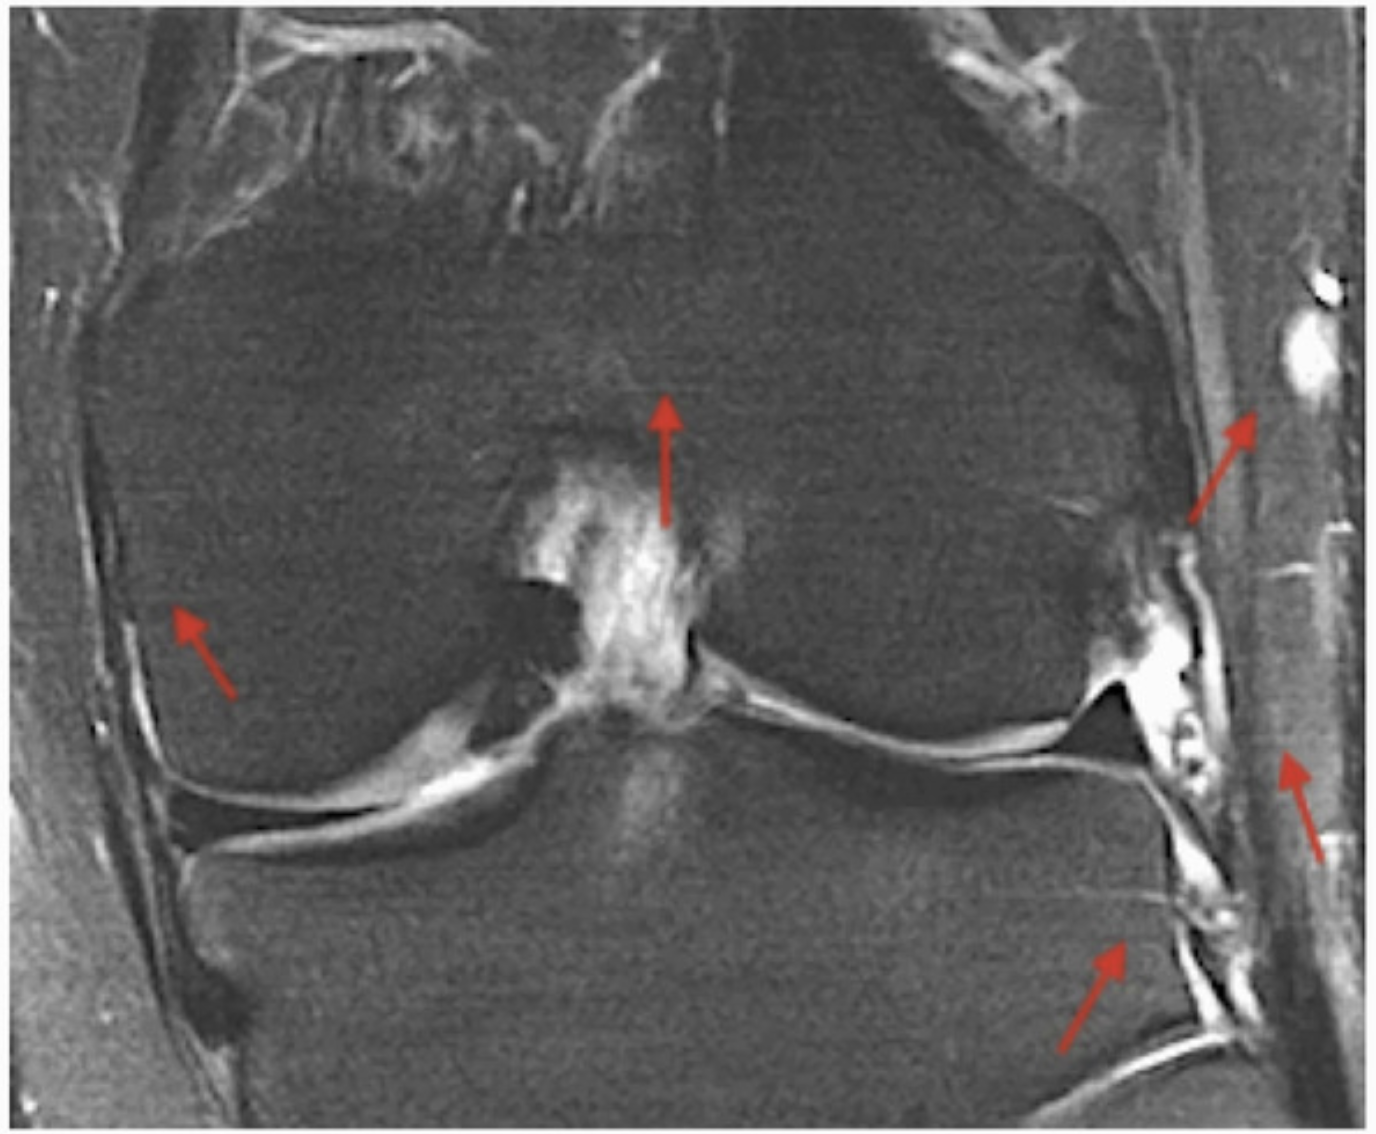
\includegraphics[scale=0.4]{neurips-2020/images/Screenshot 2020-12-15 at 09.25.34.png}
    \caption{Examples of banding artefacts presented on a reconstruction using "cascade of U-Nets" type of approach. Some of the artefacts are pointed with errors but actually they are everywhere on the image.}
    \label{fig:banding_arts}
\end{figure}

{\bf Note:} these artefacts are particularly evident for scans taken with 1.5T machines due to their additional noise. \\

{\bf Observation:} the direction striking artefacts is aligned with the direction of Cartesian undersampling. Hence if undersampling direction is changed by 90 degrees, horizontal artefacts will turn into vertical ones. \\

{\bf Method:} the full pipeline in presented on fig. \ref{fig:adversaria_art_removal_pipeline}. The main idea is to train a model with an adversarial component, where the discriminator network will distinguish between different directions of artefacts. 
For that, k-space can be transposed during the data preparation process (while the orientation of the image is preserved). \\

\begin{figure}[h!]
    \centering
    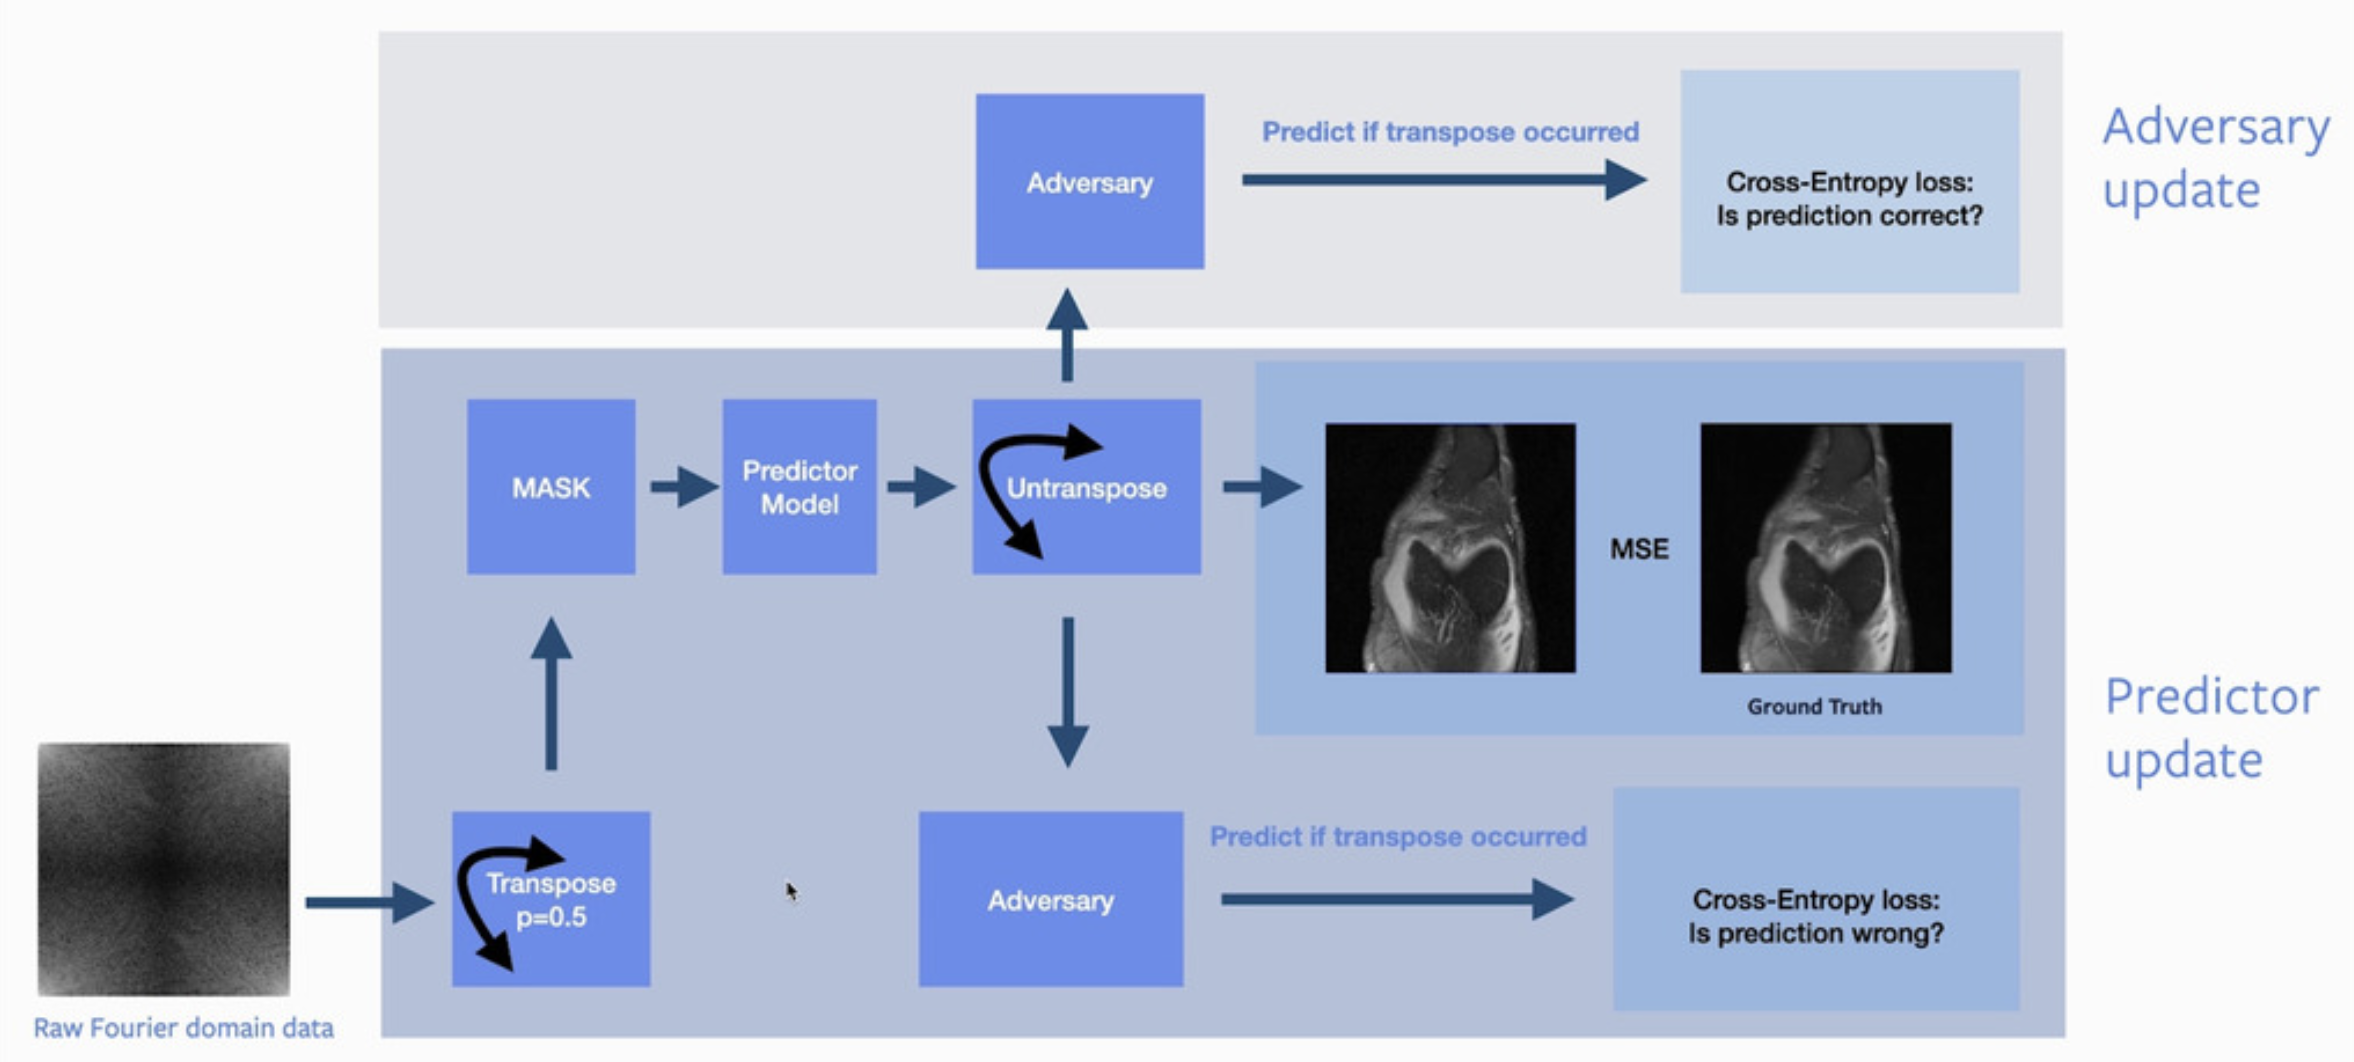
\includegraphics[scale=0.4]{neurips-2020/images/Screenshot 2020-12-15 at 09.34.10.png}
    \caption{Illustration of the full pipeline. Initial raw k-space data can is transposed with $p = 0.5$ and then fed into any reconstruction model. Next, transposed images are reverted back to the normal orientation and together with not transposed ones are fed into a discriminator network. Together with the initial supervised loss, adversarial loss in used to optimize reconstruction model. The proposed system can be trained end-to-end.}
    \label{fig:adversaria_art_removal_pipeline}
\end{figure}

{\bf Results:} the proposed technique produces outputs with little is any banding artefacts (fig. \ref{fig:result_adv_art_removal}).

\begin{figure}[h!]
    \centering
    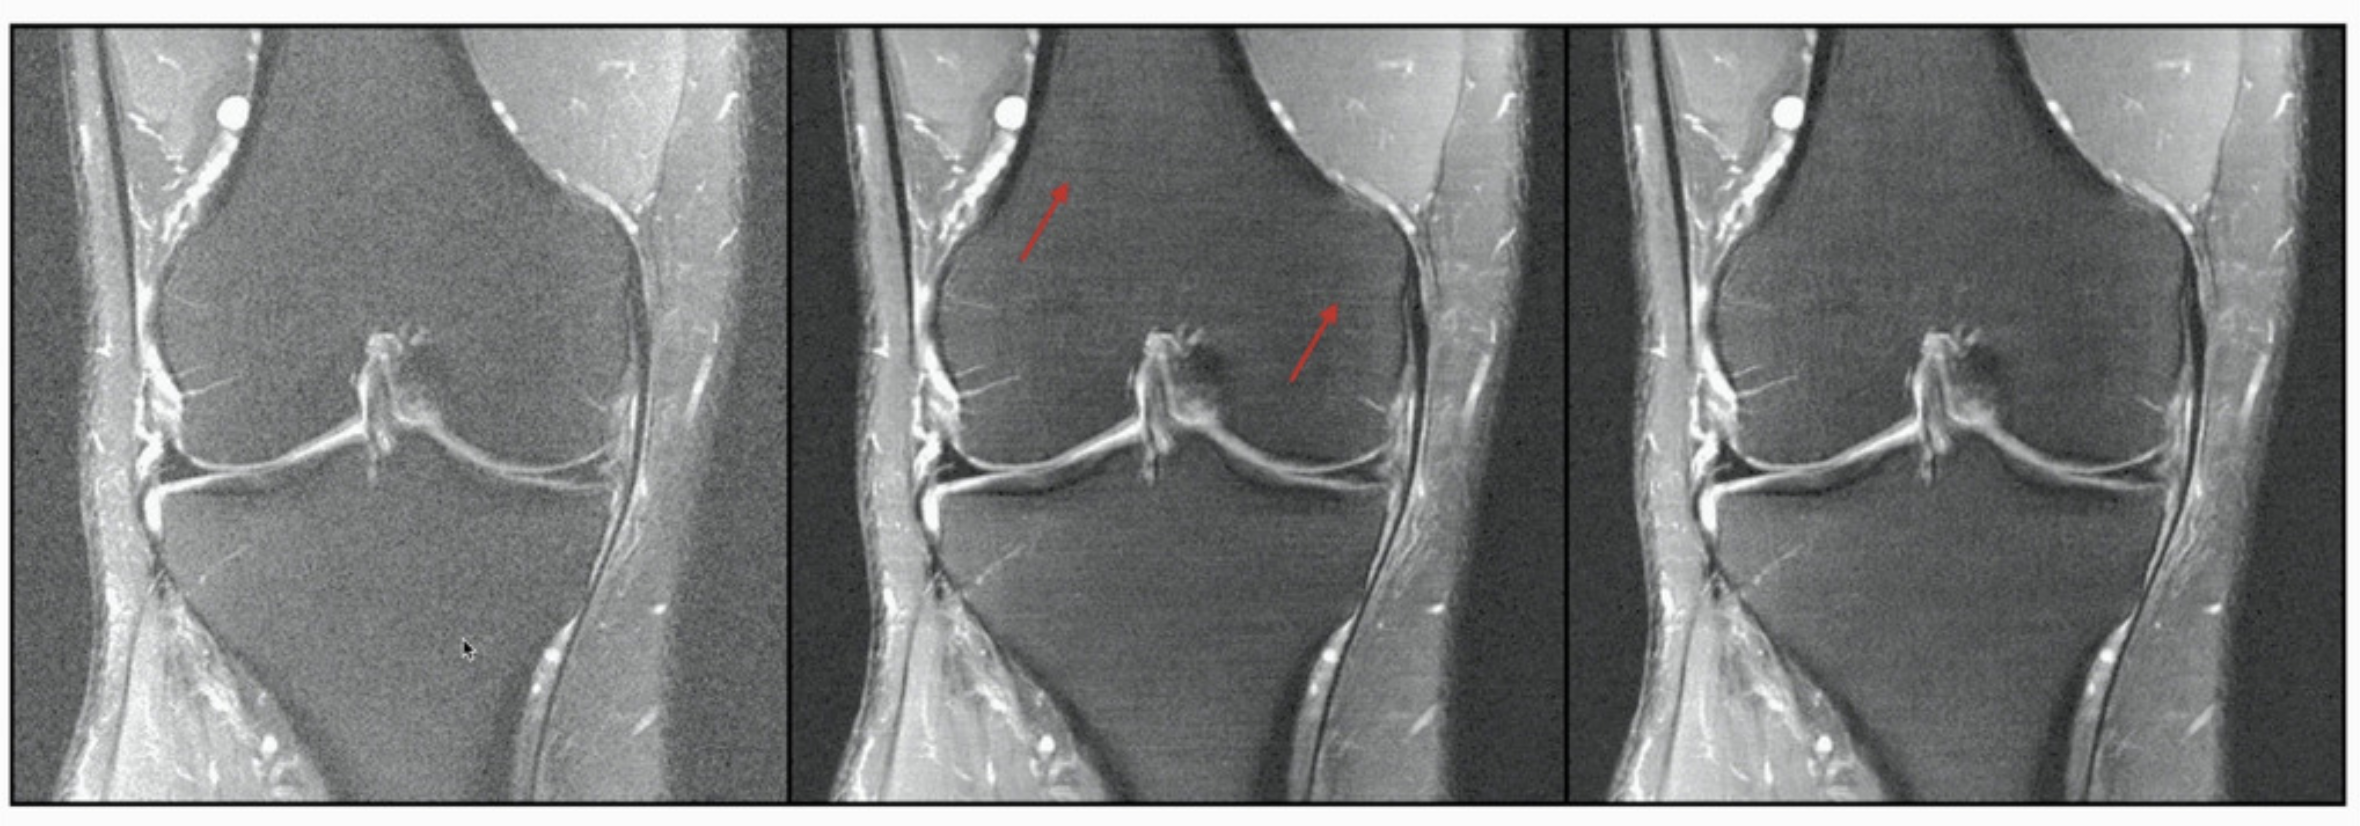
\includegraphics[scale=0.4]{neurips-2020/images/Screenshot 2020-12-15 at 09.45.10.png}
    \caption{Illustration of results from the proposed artefacts removel system. From left to right: fully sampled ground truth image (no artefacts), output of the standard model (artefacts are present), output of the proposed system trained with the adversarial component (less artefacts).}
    \label{fig:result_adv_art_removal}
\end{figure}


% ---------------
% -- Wednesday --
% ---------------
\newpage
\section{Wednesday, December 9th}
\subsection{Session: Deep Learning}

This section appeared to be quite diverse on topics and it was hard to understand the flow. However, there still were a couple of talks that I found to be interesting.

\spacerule
\subsubsection{Spotlight: What if Neural Networks had SVDs? \cite{mathiasen2020neural}}

Talk by \textit{Alexander Mathiasen}. \\

{\bf Motivation:} the SVD allows faster computation of some matrix operations commonly used by Neural Networks: 
\begin{itemize}
  \item Spectral Normalization \cite{MiyatoKKY18} - a very popular technique to stabilize training of Generative Adversarial Networks (GANs)
  \item matrix inverse and Cayley transform - essential to train flow-based models (type of generative models, alternatives to GANs) \cite{kingma2018glow}
  \item other applications such as matrix determinant and matrix exponential are less practical
\end{itemize} 

{\bf Observation:} computation of SVD can be included in the computation of gradient descent. 
In this case, getting SVD results from a layer will take no time (because values are already computed when a user asks for them). \\

{\bf Problem:} SVD cannot be directly directly formulated as a part of gradient descent step: 
\begin{equation} 
  \hat{M} \neq M - \eta\nabla_{M}
\end{equation} 

{\bf Method:} develop the Fast Householder Multiplication (FastH) method, which is a modification of the Householder transformation that supports parallel execution to better utilize GPU resources and includes some linear algebra tricks. \\

{\bf Conclusions:} new method is fast on small matrices and also his complexity grows very slowly with grows of size of the decomposed matrix: \\
\begin{center}
  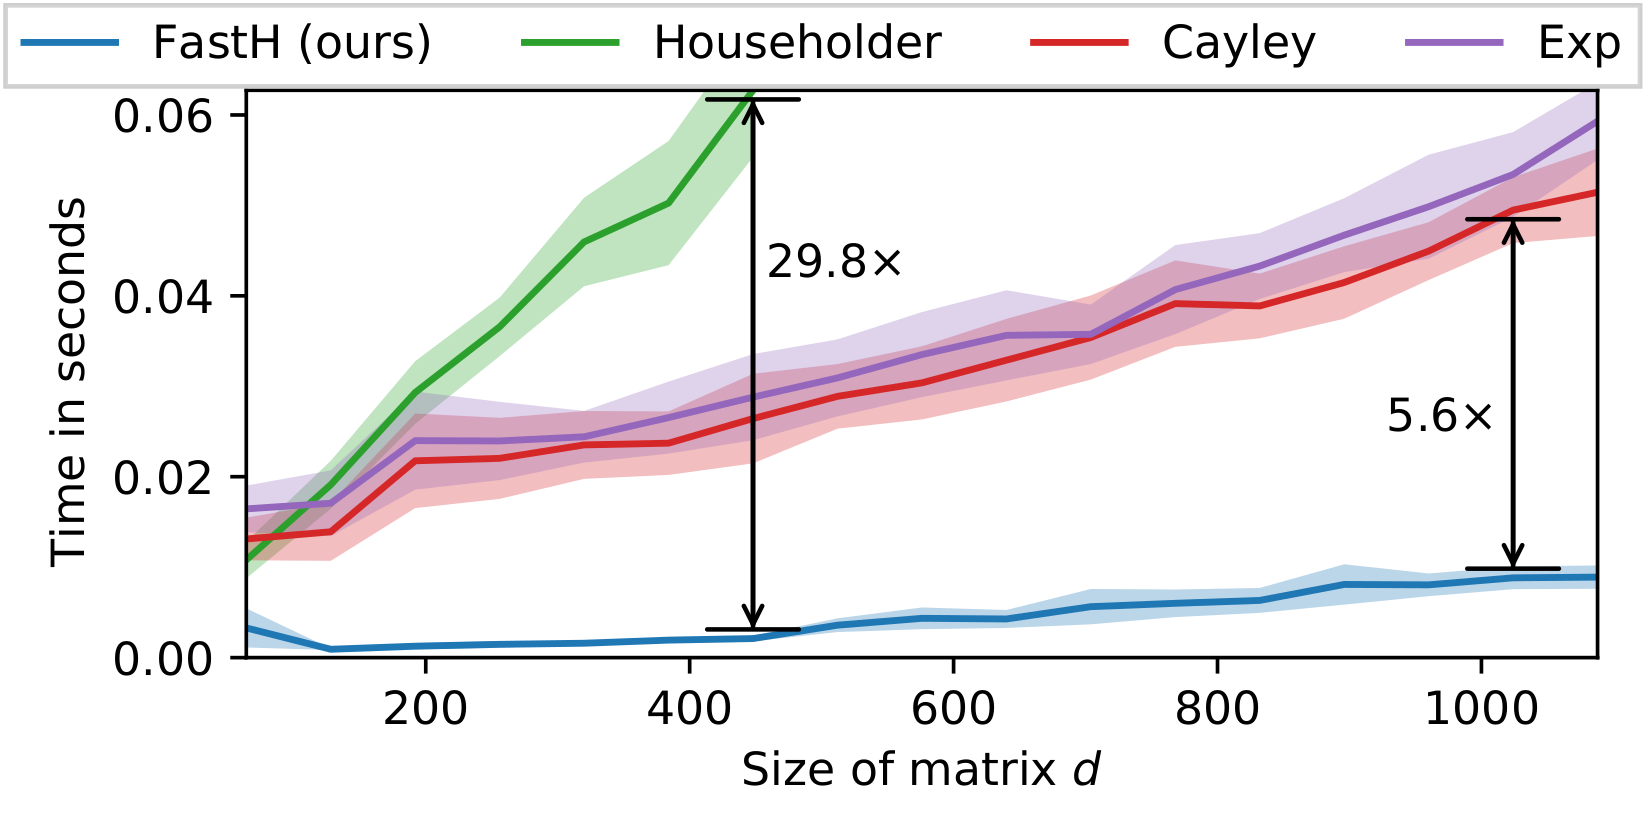
\includegraphics[scale=0.2]{neurips-2020/images/fastH.png} \\
\end{center}

{\bf Key takeaway:} \href{https://github.com/AlexanderMath/fasth/}{code in released on GitHub}, try it out. \\


\subsubsection{Spotlight: Triple descent and the two kinds of overfitting: where & why do they appear? \cite{dascoli2020triple}}

Talk by \textit{Stéphane d'Ascoli}. \\

{\bf Motivation:} when we increase the number of parameters in a machine learning model we expect loss function to decrease and then increase following the U-shape curve following the systematic bias-variance trade-off. When we increase the dataset size we expect train loss value to diminish and generalization to improve.
However, this not something that happens in real Deep Learning. \\

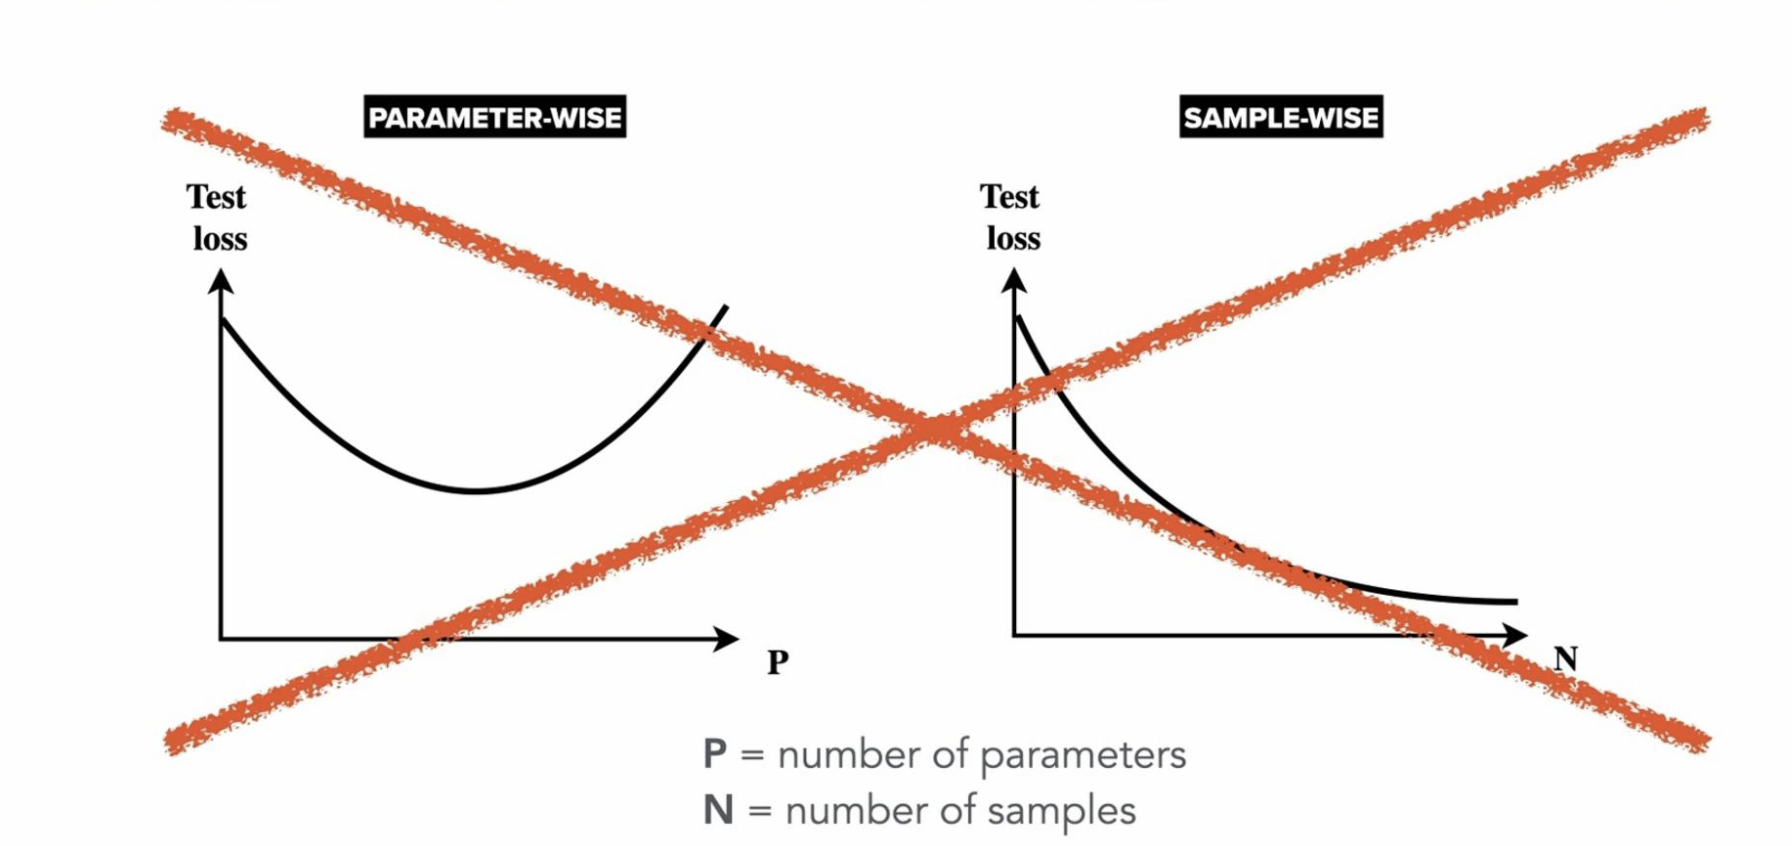
\includegraphics[scale=0.25]{neurips-2020/images/Screenshot 2020-12-09 at 18.45.09.png}
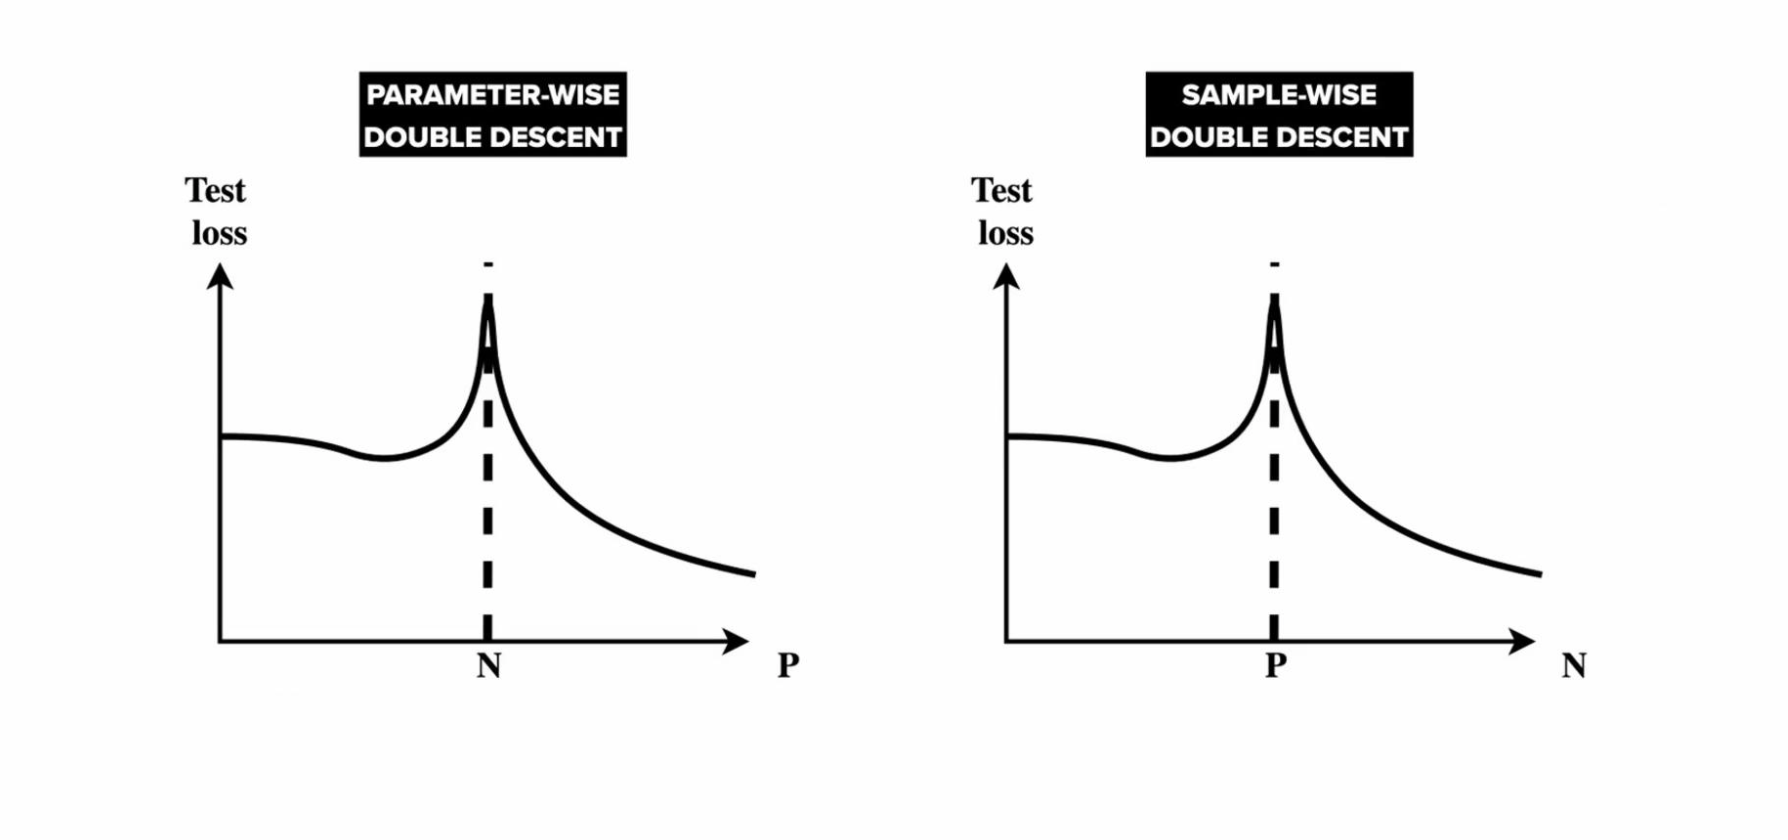
\includegraphics[scale=0.25]{neurips-2020/images/Screenshot 2020-12-09 at 18.48.59.png} \\

In this work authors focus on the sample-wise double descent curve. It was discovered in 2018 by Belkin et. al. \cite{belkin2019reconciling} and the over-fitting peak happen to co-inside with the interpolation threshold whether training loss becomes non-zero. Much earlier similar phenomena was discovered for linear models (perception) [LeCun et. al., 1991]. \\

{\bf Observation:} the non-linear peak occurs when number of training parameters $P$ is of the same order as the number of training examples $N$. However, in linear model the over-fitting peak occurs when $N$ is of the same order as input dimension $d$. Morevoer, in case of noisy regression task with weakly non-linear activation functions both peaks can be observed simultaneously. \\ 
\begin{center}
  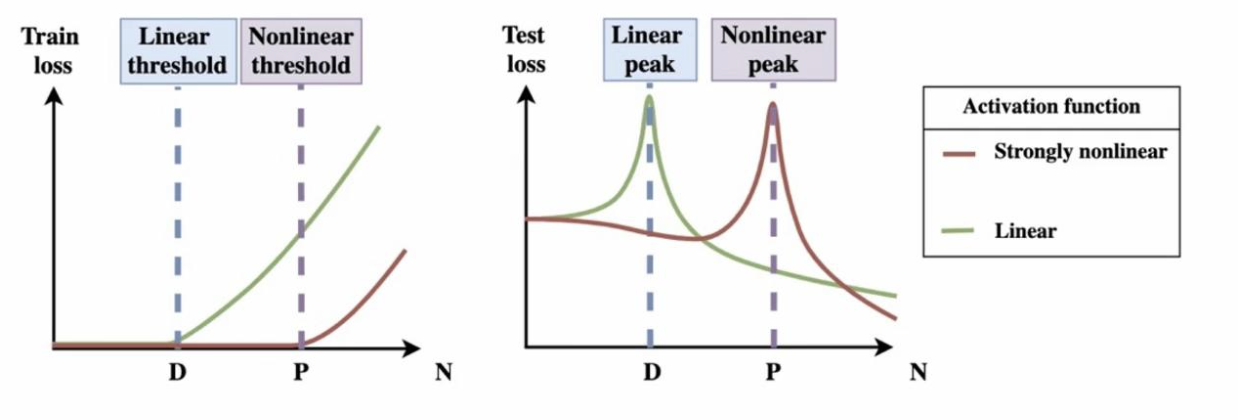
\includegraphics[scale=0.5]{neurips-2020/images/Screenshot 2020-12-09 at 19.14.11.png} \\
\end{center}

{\bf Goal of the work:} understand what cause these peaks. \\

{\bf Method:} vary degree on non-linearity of activation functions, analyse eigenvalues of Gramm matrices of tested models (fully connected).

{\bf Conclusions:} 
\begin{itemize}
  \item Linear peak is caused by the variance due to the noise in the labels
  \item Non-linear peak occurs due to initialization of random features
\end{itemize}
The consequence of this is that even if there is no noise in labels, non-linear peak when $N$ equal to $P$ still occurs, whereas the linear peak vanishes. \\

{\bf Key takeaway:} this explains why in Deep Learning we experience over-fitting even there is no noise in the dataset. \\



\subsection{Session: Social/Adversarial Learning}
\subsubsection{Spotlight: Guided Adversarial Attack for Evaluating and Enhancing Adversarial Defenses \cite{SriramananABR20}}

Talk by \textit{Gaurang Sriramanan}. \\

{\bf Motivation:} current SOTA PGD attack may not be effective due to the non-convex nature of many Machine learning tasks leading to correct response from the model under attack. Existing modifications such as performing PGD attack sequentionally with respect to several targets introduces additional computational cost. \\

{\bf Observation:} better selection of initial gradient direction leads to a stronger attack. \\

{\bf Method:} introduce the new attack called Guided Adversarial Margin Attack (GAMA):

\begin{equation}
    L = -f^{y}_{\theta}(\tilde{x}) + \max_{j \neq y} f^{j}_{\theta}(\tilde{x}) + \lambda \cdot ||f_{\theta}(\tilde{x}) - f_{\theta}(x))||^2_2 
    \label{eq:gama}
\end{equation}

First two terms of equation \ref{eq:gama} correspond to the maximum margin loss in probability space. Next, there is a smoothing term, which is represented as L2 distance between probability vectors of clean image and the perturbed image. \\

{\bf Observation:} introduction of a relaxation term (regularization) leads to smoother loss function (more convex problem) and hence better outcome of the attack. \\

\begin{figure}
  \centering
  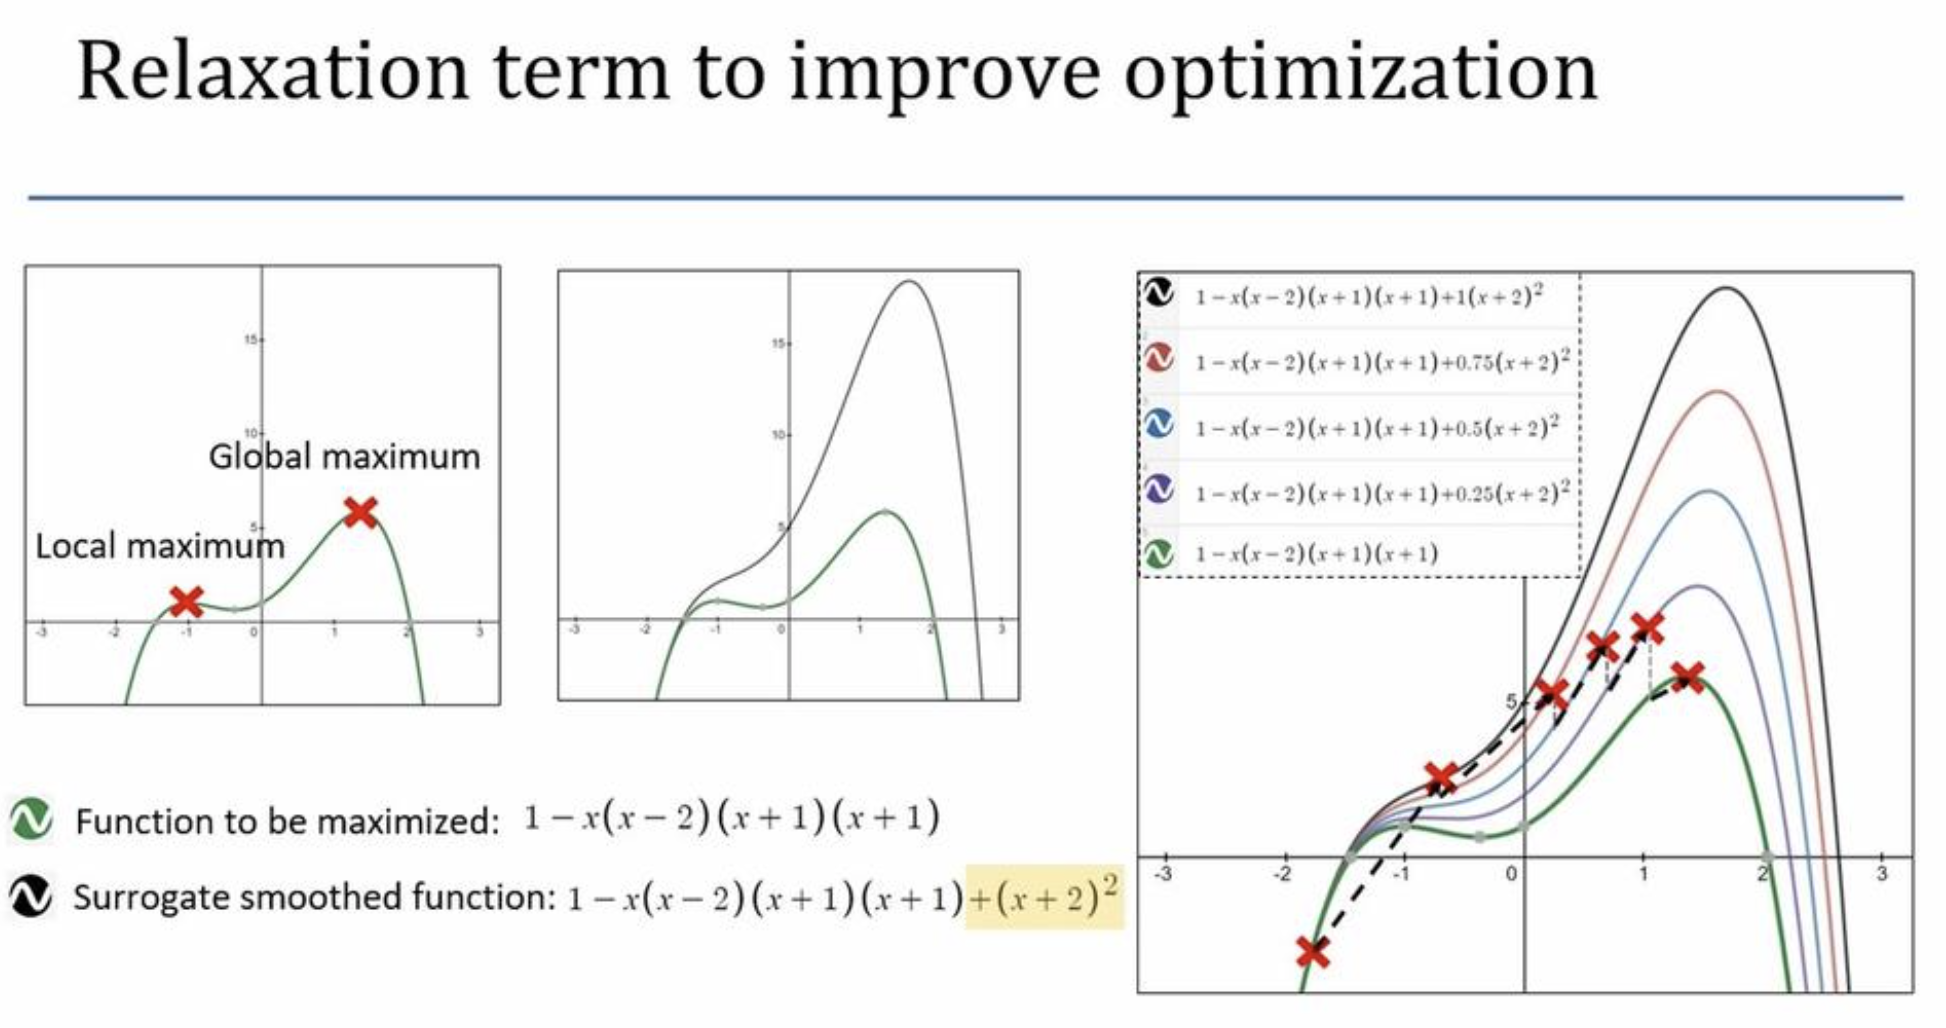
\includegraphics[scale=0.3]{neurips-2020/images/Screenshot 2020-12-10 at 21.11.50.png}
  \caption{1D example problem, which becomes more convex with introduction of the relaxation term. Loss surface becomes smoother hence leading to easier optimization and stronger attack.}
\end{figure}

{\bf Side note:} the requlization term is added with $\lambda$ parameter, which decays over optimization process and zeros-out at the end hence not effecting the ability of the system to reach an optimal solution. \\

{\bf Results:} stronger attacks with lower number of iterations (100 iterations are considered for almost all experiments in the paper). GAMA attack is tested not only against plain models, but also against current SOTA defences. \\

{\bf Key takeaways:} simple yet effective idea. The only disadvantage - only applicable for classification task, which limits its adoption in broader range of applications. \\









\subsection{Poster Session 4}
\subsubsection{Experimental design for MRI by greedy policy search \cite{BakkerHW20}}

Presented by \textit{Tim Bakker} \\

{\bf Motivation:} move away from handcrefted sampling masks towards learned aquisition strategies. \\

{\bf Observation:} the problem can be solved by joint optimization of some sampling scheme generator and the following reconstruction model. 
However, it leads to non-adaptive sampler: decision on which k-space lines to sample is made ones and not adjusted based on quality of recons made on partially sampled data. 
RL-based approach allows to make sampling scheme generation to be more adaptive. \\

{\bf Method:} an initial subsampling of k-space is obtained from the ground truth image.
The subsampled frequency domain is fed into a reconstruction method, which for neural network based reconstructions starts with an inverse Fourier transform. This intermediate step results in a zero-filled reconstruction.
The high-resolution reconstructed MR image is input to the policy network, which outputs a discrete probability distribution that represents the suggested sampling policy.
A action is sampled from this policy, corresponding to a measurement of k-space.
This measurement is simulated from the ground truth MR image, and the procedure is repeated until the acquisition budget is exhausted.
The reward of an acquisition step is given by the improvement in Structural Similarity Index of the ground truth and reconstruction resulting from that acquisition. \\

\begin{center}
  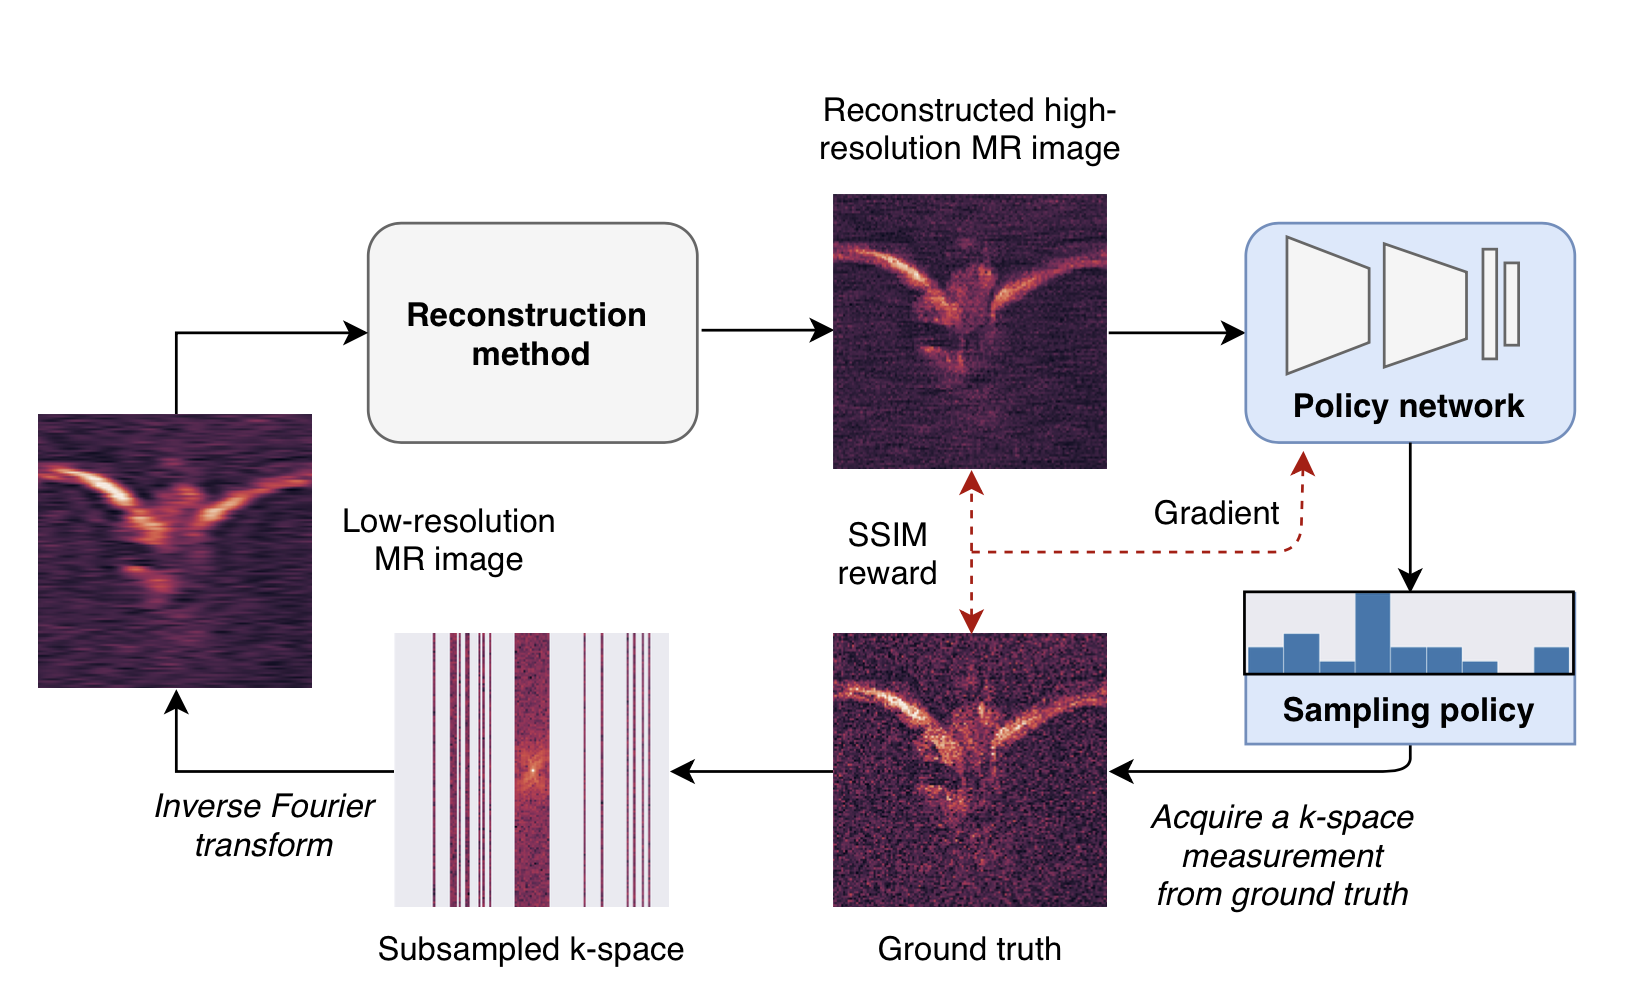
\includegraphics[scale=0.4]{neurips-2020/images/Screenshot 2020-12-10 at 11.12.09.png} \\
\end{center}

{\bf Side note:} of the biggest practical disadvantages of the approach is that reconstruction model is applied after each action $a$ meaning that several dozens of reconstruction may need to be performed before the desired resulting reconstruction is obtained. \\

{\bf Results:} results were only estimated base on SSIM values, no manual comparison with application specialists is done.
\begin{itemize}
    \item Based on SSIM values, Greed model performs better compared to other models. Learned policy was also compared with Random strategy that shares the initial mask with the other methods, and subsequently obtains a uniformly random measurement every acquisition step, similar to a simple VDS heuristic \cite{Lustig2007SparseMRI}
    \item The Greedy model is furthermore much less computationally expensive to train than any of the non-greedy models
    \item The Greedy model shows that it is adapting its predictions to individual MR images by outperforming the NA Oracle (selects as a measurement candidate in each acquisition step the column that leads to the greatest average SSIM improvement over the test dataset).
    This suggests that adaptivity is indeed a useful property for subsampling models to possess, and that this information can be learned in practice
    \item Method is verified for the single-coil case.
    It may be interesting to extend the work to more clinically relevant multi-coil case
\end{itemize} \\

{\bf Q\&A session with \textit{Tim Bakker}}

\textbf{Q:} How much is your learned policy better then some predefined one that people typically use?  
    
\textbf{A:} We have not made this comparison yet but there is a feeling that only application specialist will see the difference (remark: they do not have application specialists/clinical scientists in their research group) \\

\textbf{Q:} How much reconstructions from different policies are visually different?  

\textbf{A:} There is a huge gap in SSIM values but it is harder estimate visual difference (remark: seems like they have not done a proper visual evaluation) \\

\textbf{Q:} In the paper you tried to learn a policy with a fixed recon model. Have you consider a joint learning?  

\textbf{A:} We have not. However, we understand that joint optimization may lead to better results. It should be confirmed though (remark: our current SDF learning approach is joint and hence may be advantageous). \\

\textbf{Q:} Have you tried more clinically relevant (lower) acceleration factors?

\textbf{A:} Not really. We stick to the fastMRI accelerations of x4 and x8 and then proceeded with higher accelerations (x32) because we were interested what will happen with the agent and reconstructions. \\

\textbf{Q:} Have you considered non-cartesian sampling schemes?

\textbf{A:} Very little, it would be honest to answer no here. \\

\textbf{Q:} What are your plans? Are you going to develop the method further? (remark: the question was asked with an intent to find out about active sampling. However, I did not mention it explicitly) 

\textbf{A:} Not really. Currently, we are exploring options for clinical application and it draws all our attention. \\


% --------------
% -- Thursday --
% --------------
\newpage
\section{Thursday, December 10th}
\subsection{Poster Session 6}

This poster session contained quite some papers related to the medicine.
Self-supervision seem to be the general trend these days.


\spacerule
\subsubsection{Differentiable Augmentation for Data-Efficient GAN Training \cite{ZhaoLLZ020}}

Presented by \textit{Shengyu Zhao}. \\

{\bf Motivation:} collecting datasets is expensive. 
However, GANs trained on limited datasets suffer from low performance because it becomes easier for discriminator $D$ to just memorize training set (overfitting). Figure \ref{fig:gan_overfitting_on_limited_data} illustrates this phenomena. \\

\begin{figure}[h!]
    \centering
    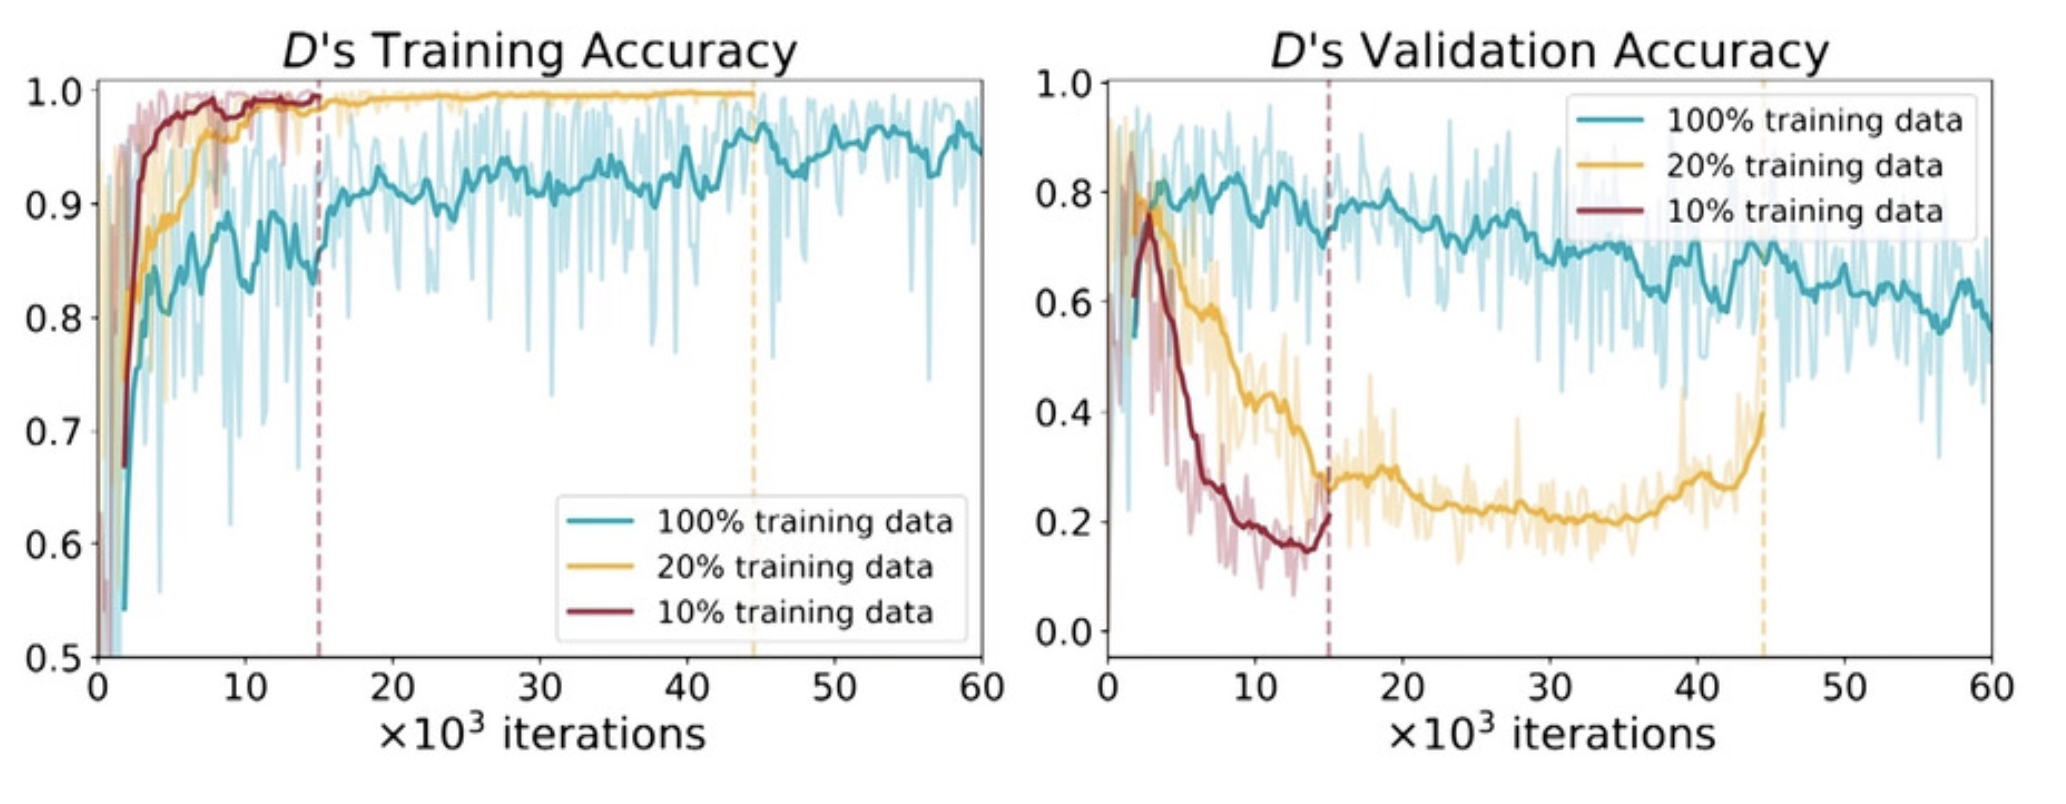
\includegraphics[scale=0.4]{neurips-2020/images/Screenshot 2020-12-11 at 10.29.55.png}
    \caption{Accuracy of the discriminator $D$ model rapidly increases when number of training samples becomes smaller. In the 20\% case training accuracy rapidly saturates while validation accuracy keeps decreasing until collapse. This phenomenon becomes more severe with only 10\% of data available.}
    \label{fig:gan_overfitting_on_limited_data}
\end{figure} 

{\bf Observation:} data augmentation can increase variability of data in case of limited datasets. \\

{\bf Problems:}
\begin{itemize}
    \item if augmentations are only introduced to the real images, outputs generated by the generator $G$ will suffer from artefacts similar to the used augmentations
    \item if augmentations are introduced to both real and fake images but used only to train $D$, it leads to even worse results because $G$ and $D$ now are trained for different tasks
\end{itemize} \\

{\bf Proposal:} introduce differentiable augmentations to modify real and fake images for both $G$ and $D$. Consider the following basic GAN definition (equation \ref{eq:gan_eq}):

\begin{equation}
  \begin{array}{l}
    L_D = \mathbb{E}_{\pmb{x} \sim p_{data}(\pmb{x})} [f_D(-D(\pmb{x}))] + \mathbb{E}_{\pmb{z} \sim p(\pmb{z})} [f_D(D(G(\pmb{z})))] \\
    \\
    L_G = \mathbb{E}_{\pmb{z} \sim p(\pmb{z})} [f_G(-D(G(\pmb{z})]
  \end{array}
  \label{eq:gan_eq}
\end{equation}

Equation \ref{eq:gan_eq} is changed to introduce differentiable augmentation $T$ as a part of the optimization problem (equation \ref{eq:gan_eq_modified}):

\begin{equation}
  \begin{array}{l}
    L_D = \mathbb{E}_{\pmb{x} \sim p_{data}(\pmb{x})} [f_D(-D(\textcolor{red}{T}(\pmb{x})))] + \mathbb{E}_{\pmb{z} \sim p(\pmb{z})} [f_D(D(\textcolor{red}{T}(G(\pmb{z}))))] \\
    \\
    L_G = \mathbb{E}_{\pmb{z} \sim p(\pmb{z})} [f_G(-D(\textcolor{red}{T}(G(\pmb{z}))]
  \end{array}
  \label{eq:gan_eq_modified}
\end{equation} 

{\bf Results:} Even trained on 20\% or 10\% of data using this method results are reasonable, FID \cite{HeuselRUNH17} scores are lower (see figure \ref{fig:diff_aug_fid}).\\ 

\begin{figure}[h!]
    \centering
    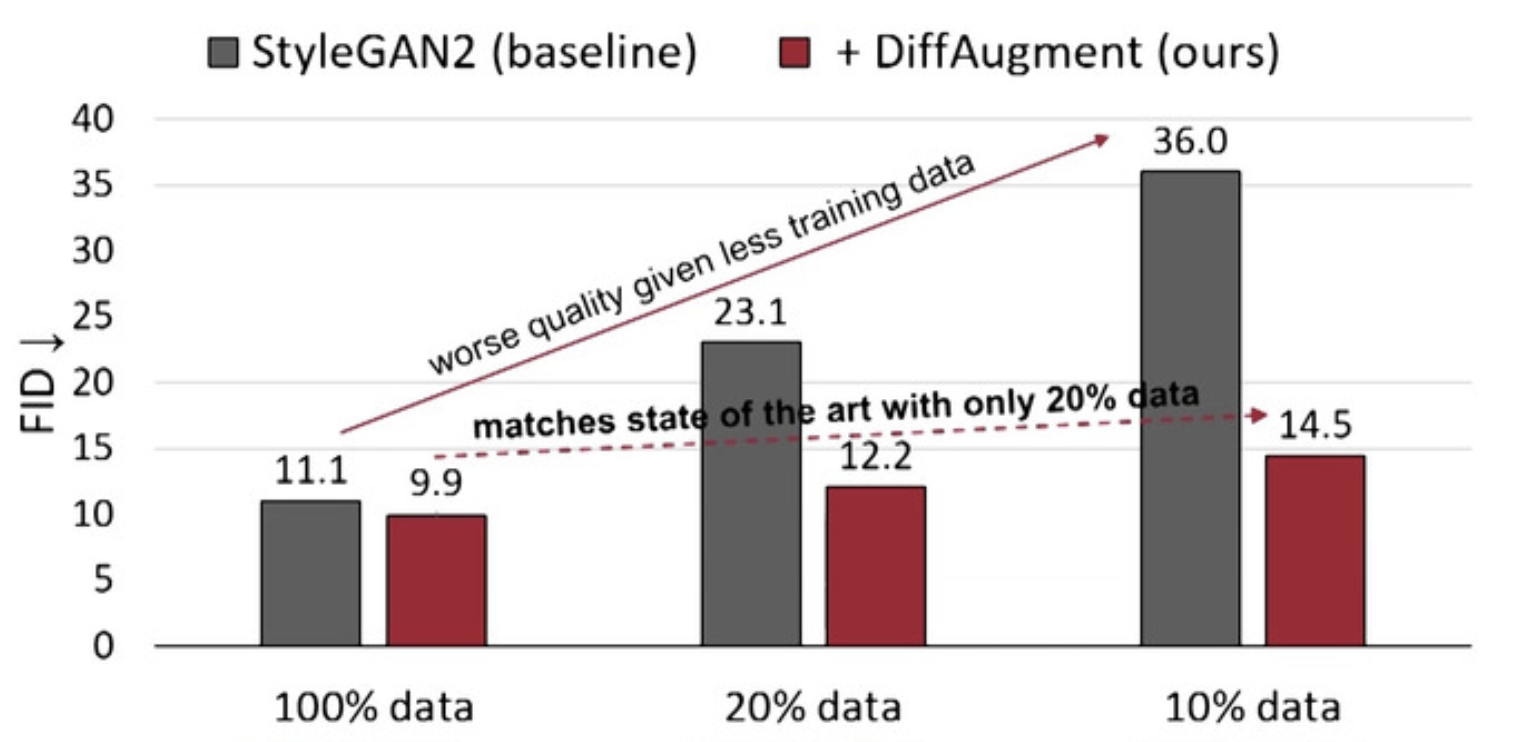
\includegraphics[scale=0.4]{neurips-2020/images/Screenshot 2020-12-11 at 10.43.05.png}
    \caption{Illustration of advantages of using differentiable augmentation on when size of available dataset is limited. Gray bins represent FID scores for GAN trained without augmentations, red bins represent the same baseline model but trained using differential augmentations.}
    \label{fig:diff_aug_fid}
\end{figure}

{\bf Key takeaways:} differentiable augmentations is in general a great idea, which is extremely useful in practice (proven by lots of independent experiments) for training GANs and other frameworks. Also code is released \href{https://github.com/mit-han-lab/data-efficient-gans}{on GitHub}.

\subsubsection{Bootstrap Your Own Latent - A New Approach to Self-Supervised Learning \cite{GrillSATRBDPGAP20}}

Presented by \textit{Jean-Bastien Grill} (also oral at the Track 27 - Unsupervised/Probabilistic)  \\

{\bf Motivation:} improve self-supervised pretraining of CNNs to provide better initialization for further fine-tuning on the end task. \\

{\bf Observation:} model can be trained not using labels from the training set. Instead, they can be generated by the network itself (its replica), which will allow to train without negative labels (potentially better performance). \\

{\bf Method:} the main features of the method are illustrated on figure \ref{fig:self_supervision_framework}. \\

\begin{figure}[h!]
    \centering
    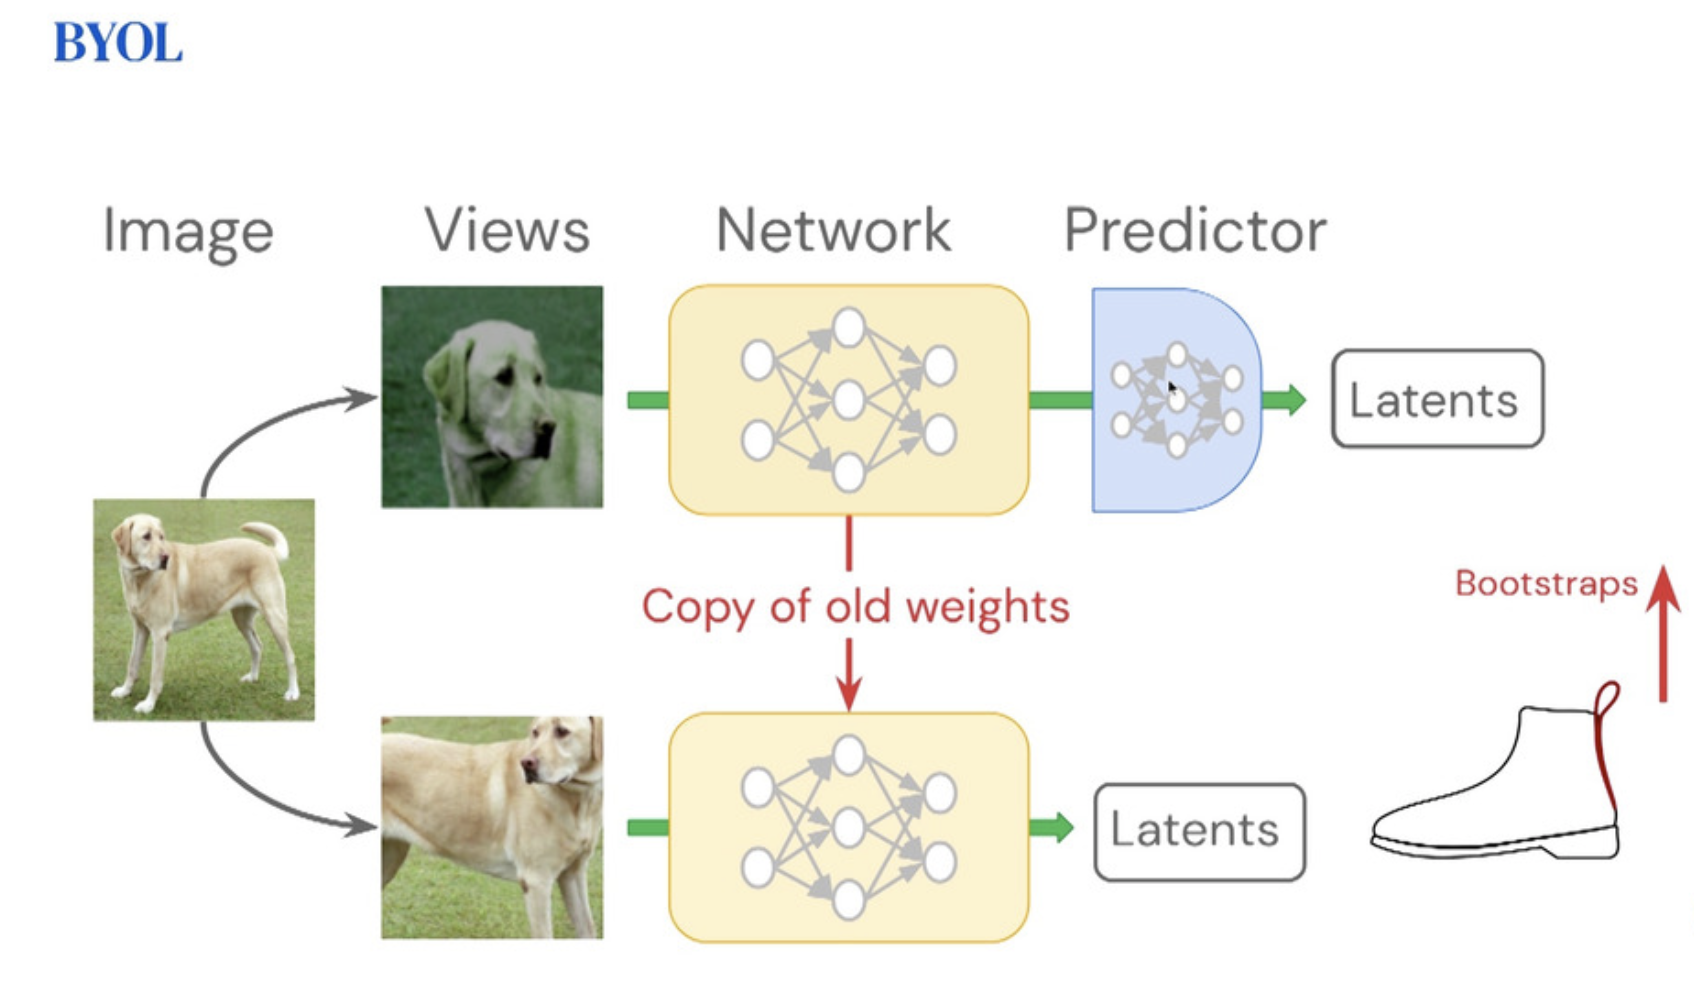
\includegraphics[scale=0.4]{neurips-2020/images/Screenshot 2020-12-11 at 19.06.09.png}
    \caption{Main elements of the BYOL method. First, two different views are extracted from an image from the training set. Second, on the views is fed into the feature extractor and next to the predictor. The predictor outputs latents, which should match bootstrapped outputs of feature extractor replica.}
    \label{fig:self_supervision_framework}
\end{figure} 

There are several key ingredient of this method:
\begin{itemize}
    \item Carefully tuned image transformations
    \item Presence of the target network (inspired by Reinforcement Learning)
    \item Additional predictor on online network (makes training more stable)
\end{itemize} 

{\bf Results:} current SOTA, more resilient to transformation and batch size than contrastive methods. \\

{\bf Key takeaways:} need to try self-supervision in other tasks (may be start with a simpler method). Code is \href{https://github.com/lucidrains/byol-pytorch}{released on GitHub}. \\



\subsubsection{Noise2Same: Optimizing A Self-Supervised Bound for Image Denoising \cite{XieWJ20}}

Presented by \textit{Yaochen Xie}.  \\

{\bf Motivation:} enhance previous SOTA self-supervided denoising model Noise2Self \cite{BatsonR19} by solving its main problem - utilization of information about center pixel without knowing the noise model. \\

{\bf Related work:} Noise2Noise \cite{LehtinenMHLKAA18} compared to the proposed approach requires more supervision with noisy-noisy pairs. Here, only unpaired noisy images are available. In Noise2Void \cite{KrullBJ19} and Noise2Self \cite{BatsonR19} \textbf{blind spot denosing} is proposed. Here, some masks are applied and then each pixel is denoised with this context. The biggest disadvantage of this approach is that only surrounding pixel are utilized while the information from the pixel being denoised is not used. This leads to lower performance. Some methods to address it were proposed by they rely on noise model, which is unknown in most cases. \\

{\bf Observation}: one term in the loss function of the Noise2Self model can be bound to be zero instead of assuming it. \\

{\bf Method:} in general, method follows the Noise2Self framework. The only difference is the objecting function. It is changed to meet zero-value requirement instead of assuming it. \\

\begin{figure}[h!]
    \centering
    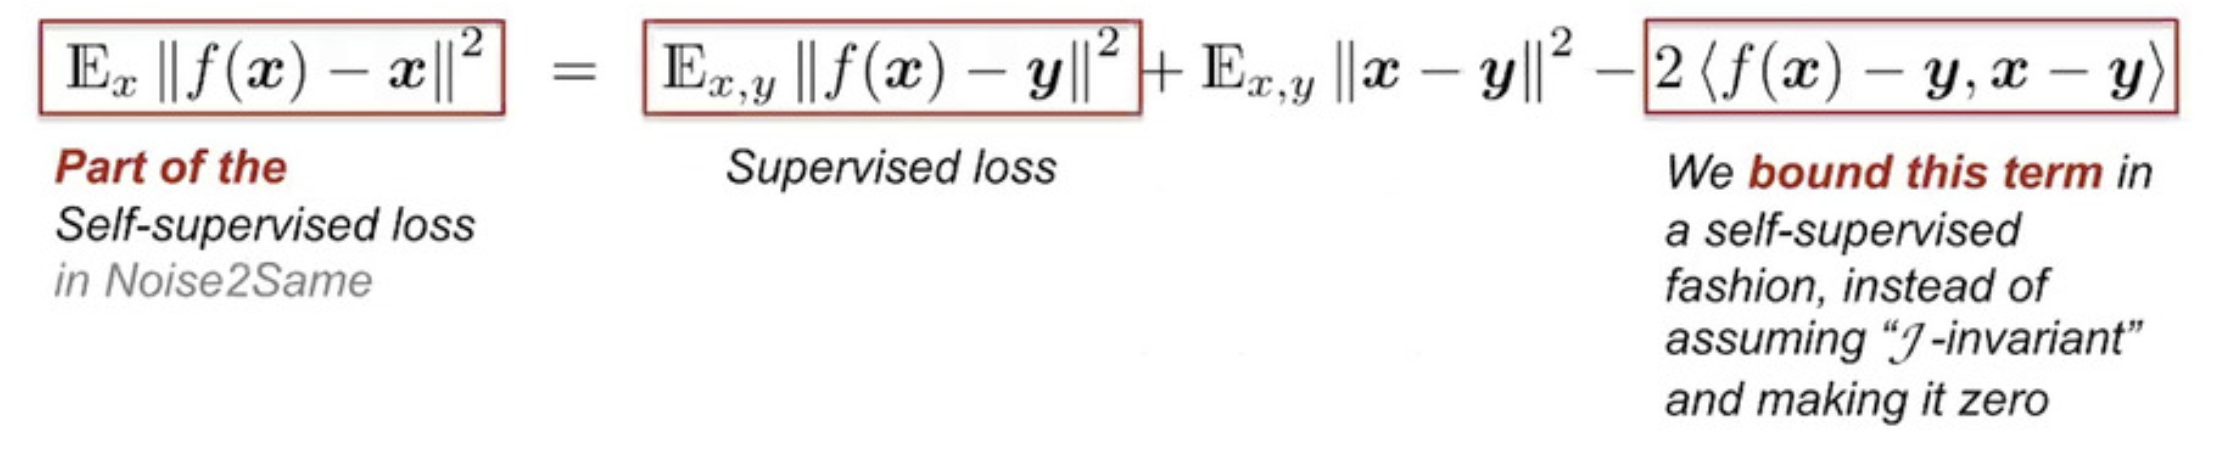
\includegraphics[scale=0.4]{neurips-2020/images/Screenshot 2020-12-12 at 14.58.30.png}
\end{figure} 

{\bf Results and takeaways:} SOTA results compared to other self-supervised/weakly supervised methods, code is \href{https://github.com/divelab/Noise2Same}{released on GitHub}. \\




\subsubsection{3D Self-Supervised Methods for Medical Imaging \cite{TalebLDSGBL20}}

Presented by \textit{Aiham Taleb}.  \\

{\bf Motivation:} most of known self-supervised method are developed for 2D data. However, there is a way to utilize 3D spacial information, which is often available in medical imaging. \\

{\bf Method:} adapt 2D self-supervied pretraining methods to 3D. The following methods are adapted: 
\begin{itemize}
    \item Contrastive Predictive Coding
    \item Rotation Prediction
    \item Relative Patch Location
    \item Jigsaw Puzzle Solving
    \item Exemplar Networks
\end{itemize} 

{\bf Results and takeaways:} not much novelty but code for the proposed 3D methods is \href{https://github.com/HealthML/self-supervised-3d-tasks}{released on GitHub}. \\

% ------------
% -- Friday --
% ------------
\newpage
\section{Friday, December 11th}
\subsection{Workshop: Workshop on Deep Learning and Inverse Problems}

Even though this workshop is dedicated to inverse problems in broad sense of this term, the majority of presentations are somehow related with imaging. 
Moreover, significant fraction of them is either dedicated to MRI reconstruction or at least somehow mention it. 
This observation underlines consensus of the research community on the importance of this problem.

\subsubsection{Uncertainty Quantification in Deep MRI
Reconstruction \cite{edupuganti2020uncertainty}}

Presented by \textit{Vineet Edupuganti}. \\

{\bf Motivation:} accelerated MRI reconstruction is unreliable, especially when generative models are applied. Need to estimate uncertainty of a reconstruction model to help radiologist to avoid mistakes. \\

{\bf Background:} most of existing approaches (Deep Ensembles \cite{Lakshminarayanan17}, VAE sampling \cite{corr/abs-2007-08128}) for epistemic uncertainty estimation leverage one or another form of the Monte Carlo sampling: several samples are utilized to compute statistics, which are then represented as results. One example of this approach is to sample from VAE and compute variance of results. However, it is impossible to compute bias without ground truth image using this method. \\

{\bf Method:} authors propose to utilize  Stein’s Unbiased Risk Estimator
(SURE) \cite{doi:10.1080/01621459.2018.1429276} to compute bias-free uncertainty estimation without reference image. For that, the following derivation is performed.

Given the ground truth image $x_0$, the zero-filled image can
be written as 

\begin{equation}
    x_{zf} = x_0 + v
\end{equation} 

where $v$ is noise. Now considering reconstruction $\hat{x}$ with
dimension $n$, one can expand test MSE as 

\begin{equation}
    \mathbb{E}|| \hat{x} - x_0 ||^2 = \mathbb{E} || x_0 - x_{zf} + x_{zf} - \hat{x} ||^2 = -n \sigma^2  + \mathbb{E} || x_{zf} - \hat{x} ||^2 + 2Cov(x_{zf}, \hat{x})
    \label{eq:sure-one}
\end{equation} 

Since $x0$ is not present in \ref{eq:sure-one}, we see that SURE serves as a surrogate for MSE even when the ground truth is unknown. 
A key assumption behind SURE is that the noise process v that relates the zero-filled image to the ground truth is normal, namely $v \sim N(0, \sigma^2
I)$. 
With this assumption SURE is formulated as follows 

\begin{equation}
    SURE = -n \sigma^2 || \hat{x} - x_zf ||^2 + \sigma^2 tr(\partial \hat{x} / \partial x_zf)
\end{equation}

\textbf{Important note:} previous assumption may not hold in practice. 

Authors show that when error in the output reconstruction is not large, and as a result $\sigma^2$ can be estimated as 

\begin{equation}
    \sigma^2 = || \hat{x} - x_{zf} ||^2  / n
\end{equation} 

This assumption allows to formulate SURE as follows 

\begin{equation}
    SURE = \sigma^2 tr(\partial \hat{x} / \partial x_zf)
\end{equation} 

\textbf{Important note:} this assumption on only holds for low acceleration rates and artefact-free reconstruction models. 
Since this method is developed for evaluation of potentially artefact-prone models, this assumption looks quite strong. \\

Further investigations are targeted on acceleration of computations of trace of the end-to-end network Jacobian, which otherwise can be problematic. 
Authors also approach the problem of the requirement for MRI noise to follow standard normal distribution. \\

{\bf Results and takeaways:} the main contribution of this work is to apply SURE to the uncertainty estimation task in the domain of medical imaging, which has not been done before. 
An example of high correlation between estimated SURE values are computed MSE error is illustrated on figure \ref{fig:sure-result}.

\begin{figure}[h!]
    \centering
    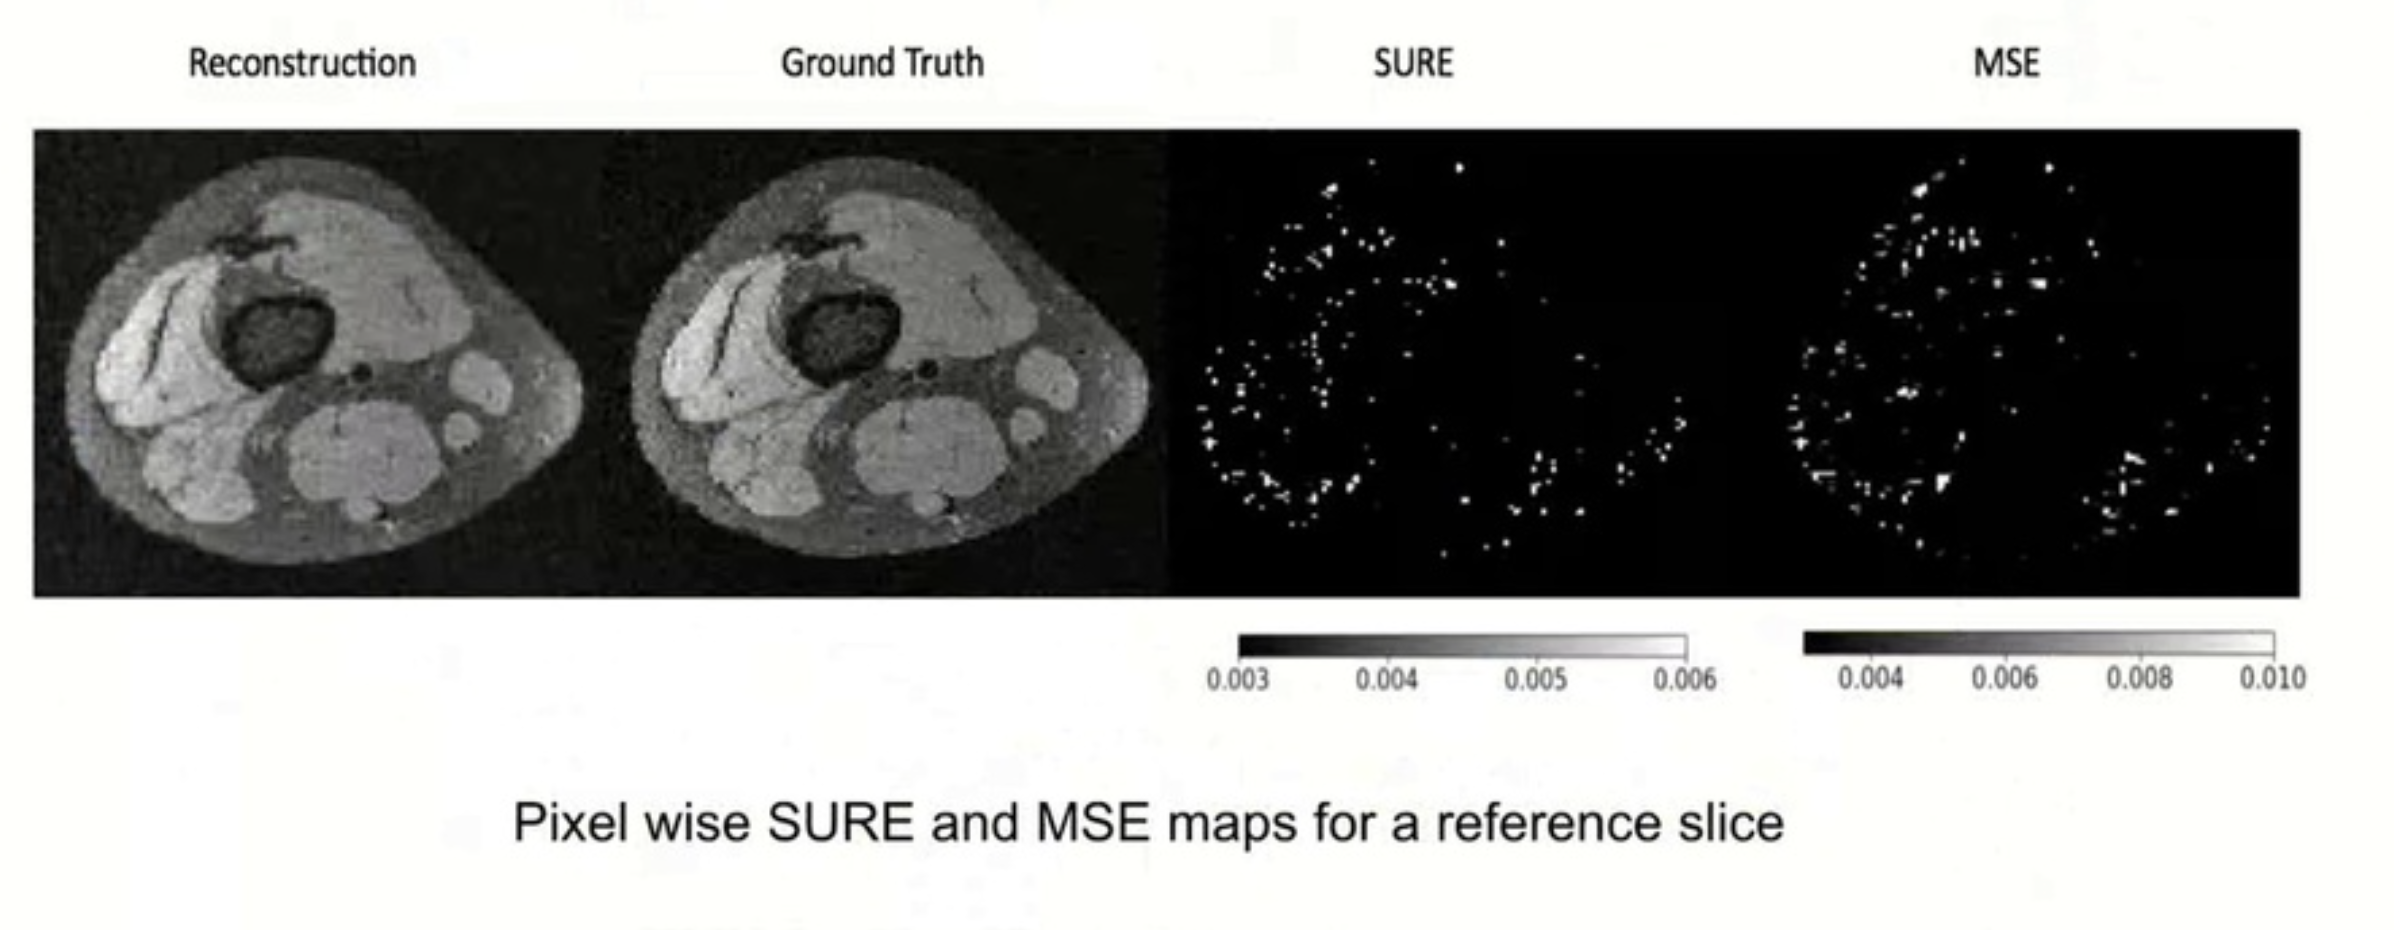
\includegraphics[scale=0.4]{neurips-2020/images/Screenshot 2020-12-12 at 17.26.28.png}
    \label{fig:sure-result}
\end{figure}





\subsubsection{Model Adaptation for Inverse Problems in Imaging \cite{gilton2020model}}

Presented by \textit{Rebecca Willett}. \\

{\bf Motivation:} having measurements $y$ and a neural network $f_{\phi}$ trained with some forward model $A_0$, make high quality reconstructions $\hat{x}$ if forward model used during inference $A_1$ is different from the one using for training ($A_0$). 
The scheme of the task setup is represented on fig. \ref{fig:inv_prob_setup}
Authors call this phenomenon a \textit{model drift}. \\

\begin{figure}[h!]
    \centering
    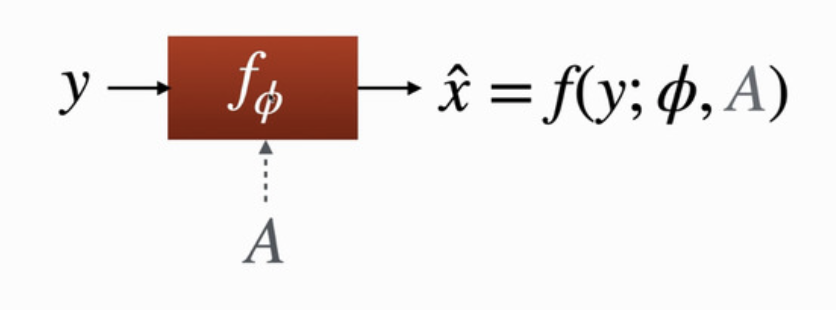
\includegraphics[scale=0.3]{neurips-2020/images/Screenshot 2020-12-13 at 20.44.08.png}
    \caption{Neural network with parameters $\phi$ (and optionally A) inputs $y$ and outputs an estimate $\hat{x}$.}
    \label{fig:inv_prob_setup}
\end{figure} 

{\bf Example:} train a fast MRI network with one acceleration rate but perform inference on some different acceleration rate. 
Even if the acceleration rate is lower, there is a domain shift that makes the network less capable to produce a high-quality estimate. \\

{\bf Definitions:} 
\begin{itemize}
    \item {\bf Distribution drift:} $p(X, Y)$ changes \textit{in unknown way} between train and deployment
    \item {\bf Model drift:} $p(X, Y)$ changes \textit{in known or partially known way} between train and deployment
    \item {\bf Domain adaptation:} first train with many samples $(x_i^{(0)}, y_i^{(0)}) \sim p_0$, then adapt using few samples from $(x_i^{(1)}, y_i^{(1)}) \sim p_1$
    \item {\bf Model adaptation:} first train with many samples $(x_i^{(0)}, y_i^{(0)}) \sim p_0$ and, then adapt using few samples from  $(?, y_i^{(1)}) \sim p_1$ (images are not known) 
\end{itemize}
\\ 

{\bf Method:} train a reconstruction network for a known forward model then adapt to a new forward model without access to ground truth images, and without knowing the exact parameters of the new forward model. \\

\underline{Proposed approaches are:}   

{\bf Parametrize and Perturb}: use calibration data to \textit{perturb} parameters of the original reconstruction network. 
In practice it means conversion of $f_0$ to some $f_1$ that will be able to handle $A_1$.

\begin{figure}[h!]
    \centering
    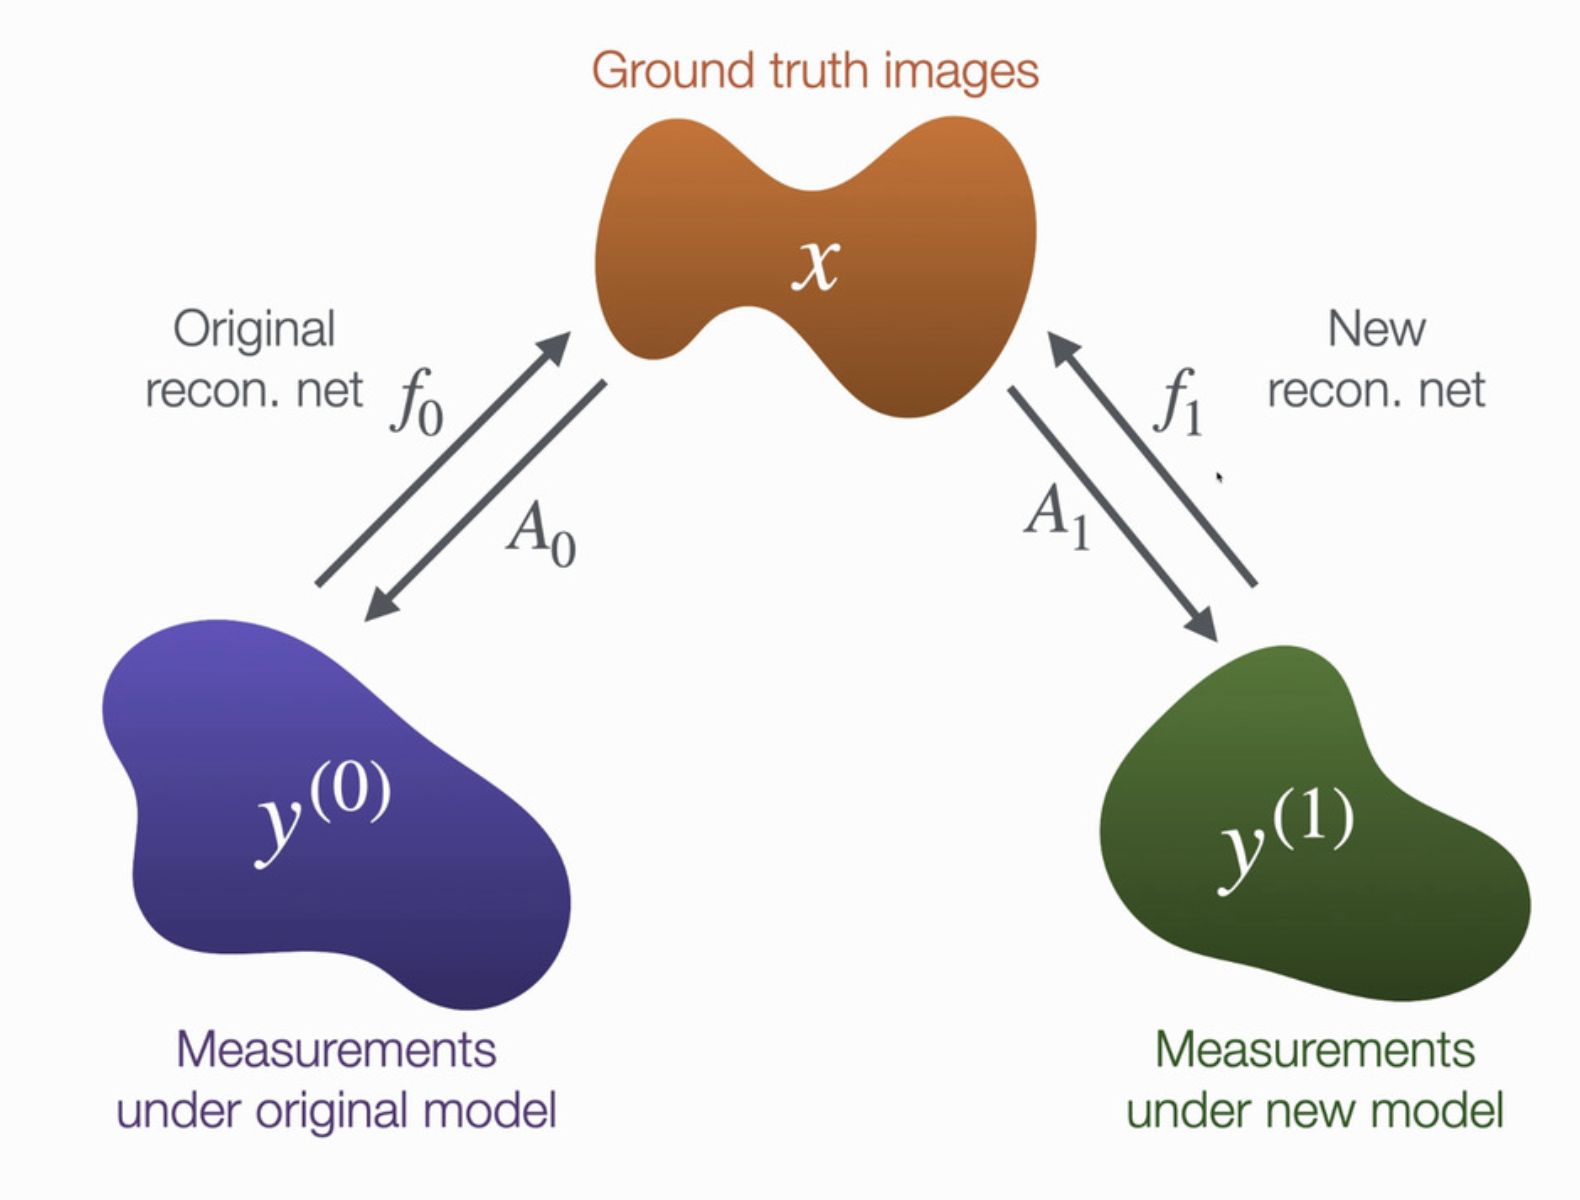
\includegraphics[scale=0.4]{neurips-2020/images/Screenshot 2020-12-13 at 21.21.21.png}
    \caption{Illustration of the Parametrize and Perturb approach. $f$ is perturbed to be able to handle $A_1$ during the inference time.}
    \label{fig:PP_approach}
\end{figure} \\

{\bf Condition and Correct}: train a new (correction) network $h_{\theta}$ to map $A_1$ to $A_0$ and then apply $f_{\phi}$.

\begin{figure}[h!]
    \centering
    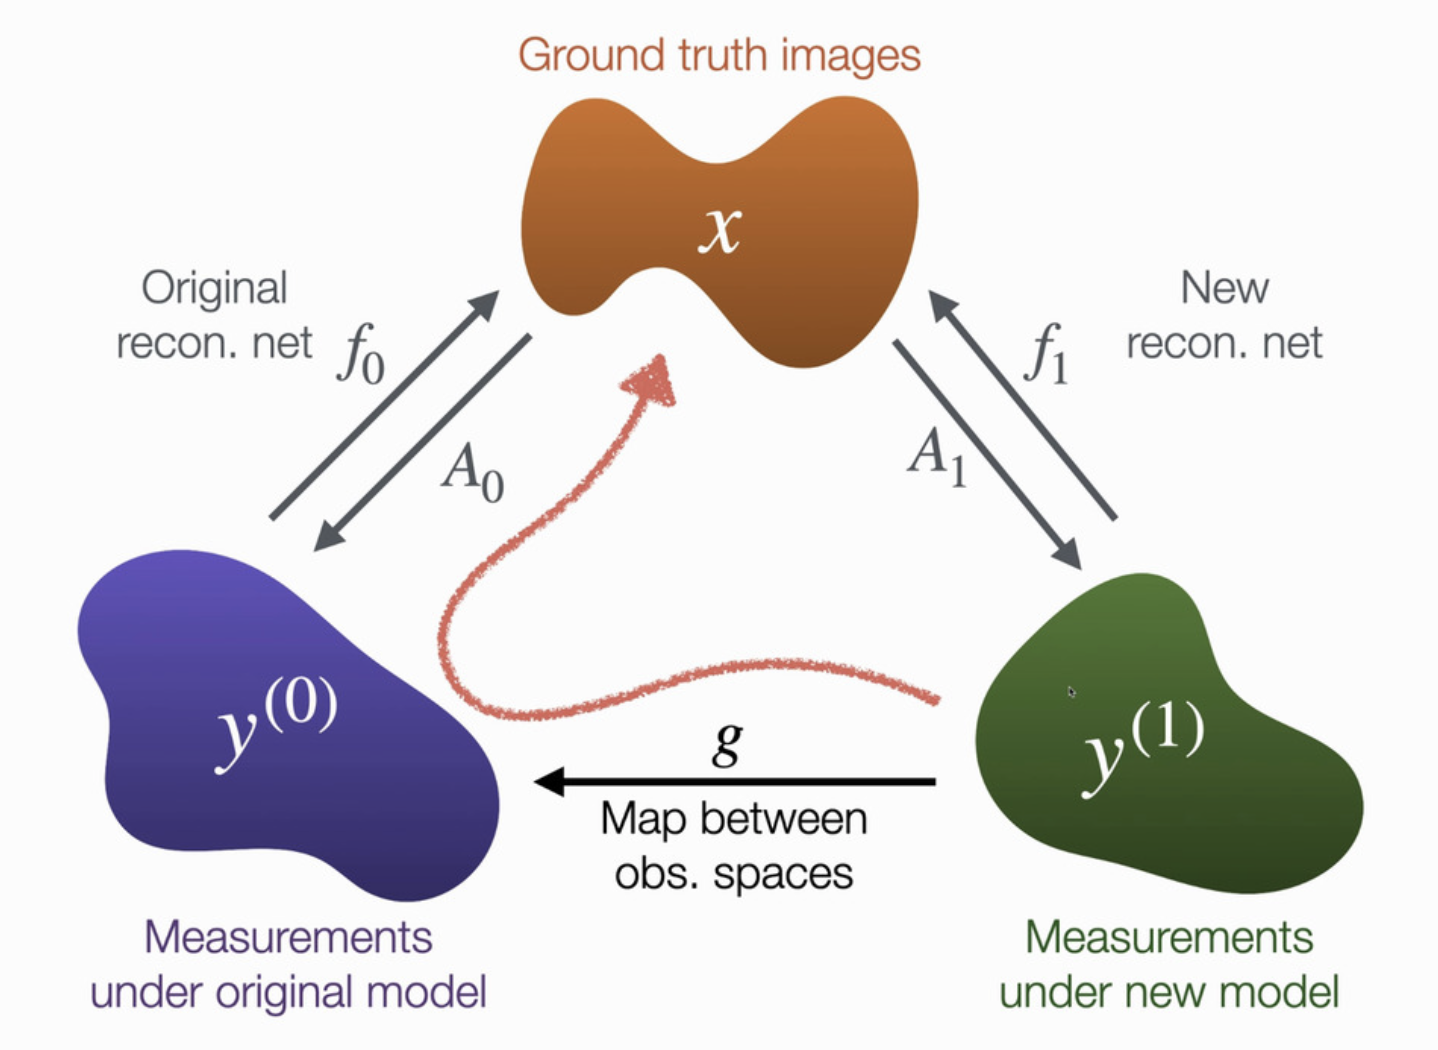
\includegraphics[scale=0.4]{neurips-2020/images/Screenshot 2020-12-13 at 21.24.26.png}
    \caption{Illustration of the Condition and Correct approach. Output of the $A_1$ is made similar to $A_0$ and then $f_\phi$ is applied}.
    \label{fig:my_label}
\end{figure}



{\bf Results:} authors show high-quality results (fig. \ref{fig:adaptation_results_11}, \ref{fig:adaptation_results_2}, \ref{fig:fast_mri_recon}, \ref{fig:moco_recon}), which confirm that their methods allow to increase the quality of resulting images if model drift takes place.
More concretely:
\begin{itemize}
    \item Condition and Correct method, in general, works a little bit better.
    \item The most significant visual improvements are presented for the motion correction problem.
    \label{fig:adaptation_results_11}
\end{itemize}

\begin{figure}[h!]
    \centering
    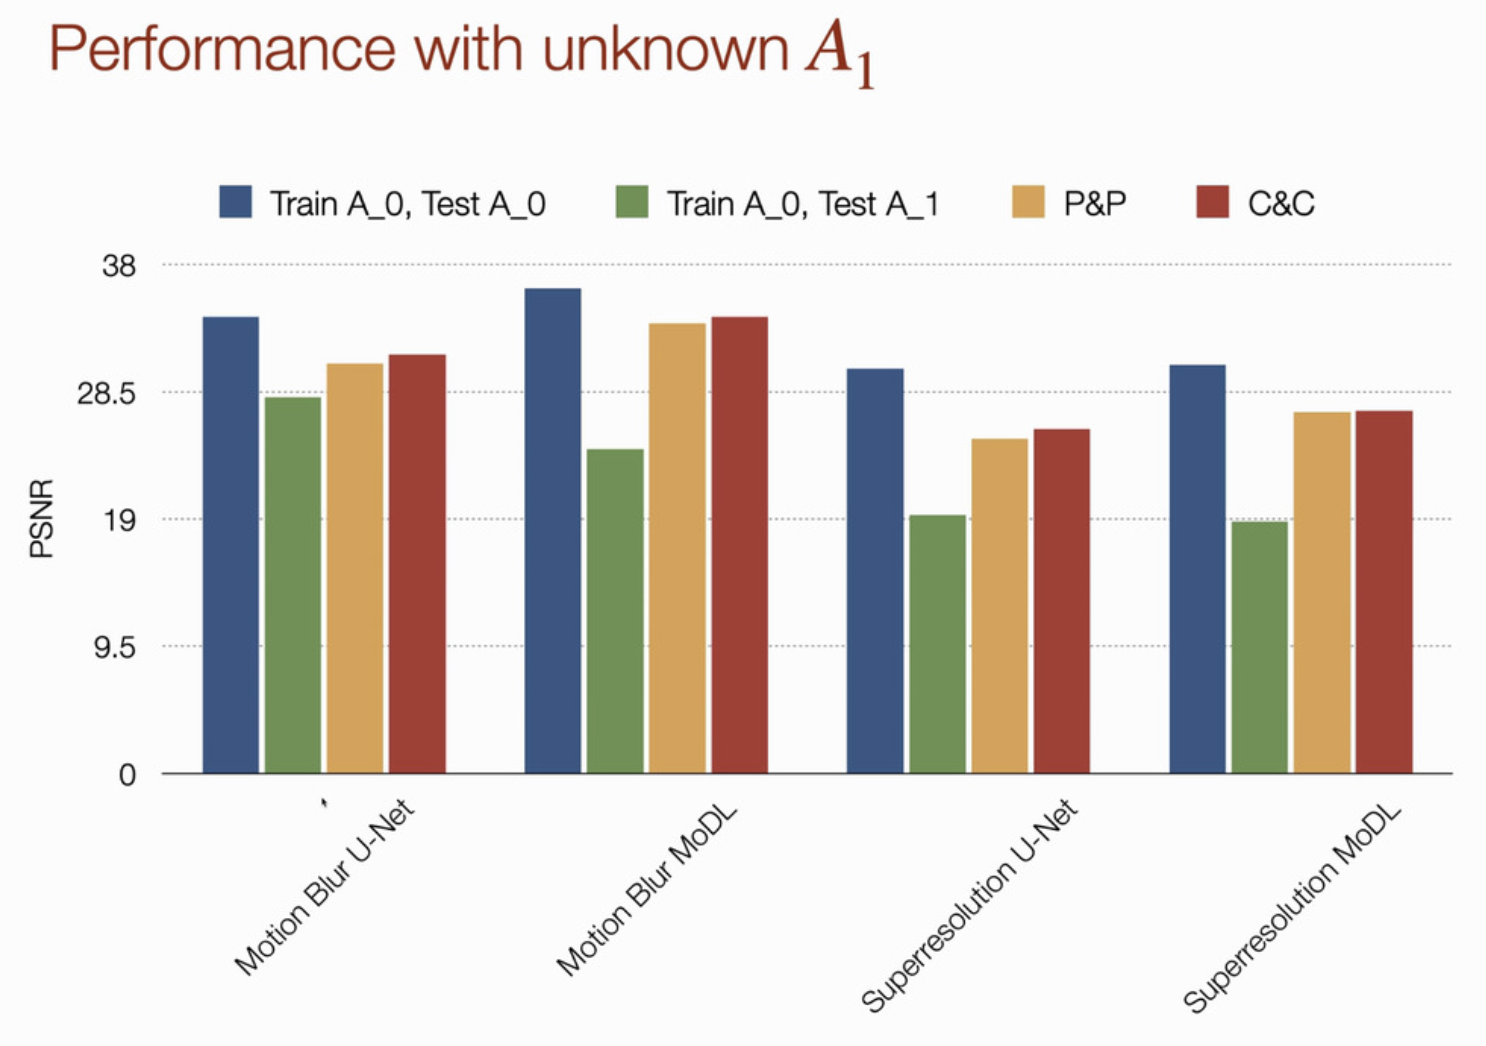
\includegraphics[scale=0.4]{neurips-2020/images/Screenshot 2020-12-13 at 21.34.45.png}
    \caption{Comparison between performance of the reconstruction model in case if $A_1$ is unknown (realistic setting) on various inverse problems.}
    \label{fig:adaptation_results_2}
\end{figure}

\begin{figure}[h!]
    \centering
    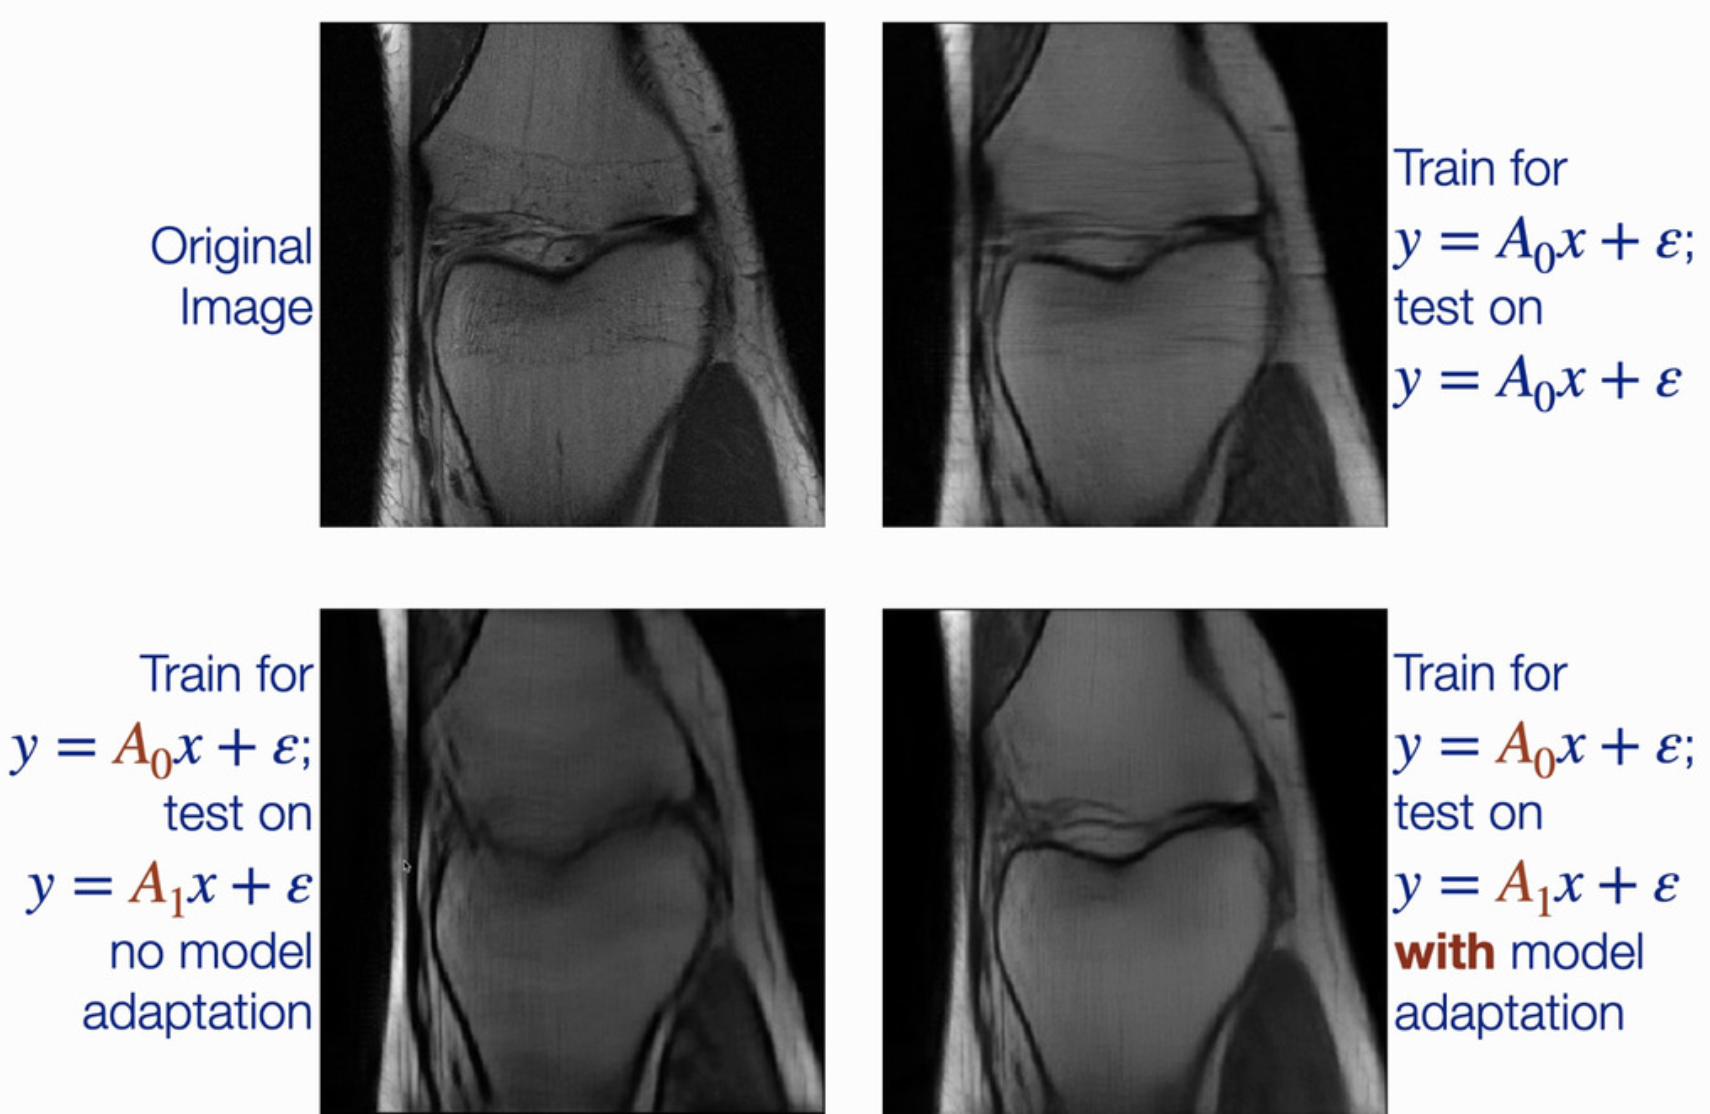
\includegraphics[scale=0.4]{neurips-2020/images/Screenshot 2020-12-13 at 21.13.23.png}
    \caption{Example of the performance of the proposed method for the fast MRI reconstruction problem}
    \label{fig:fast_mri_recon}
\end{figure}

\begin{figure}[h!]
    \centering
    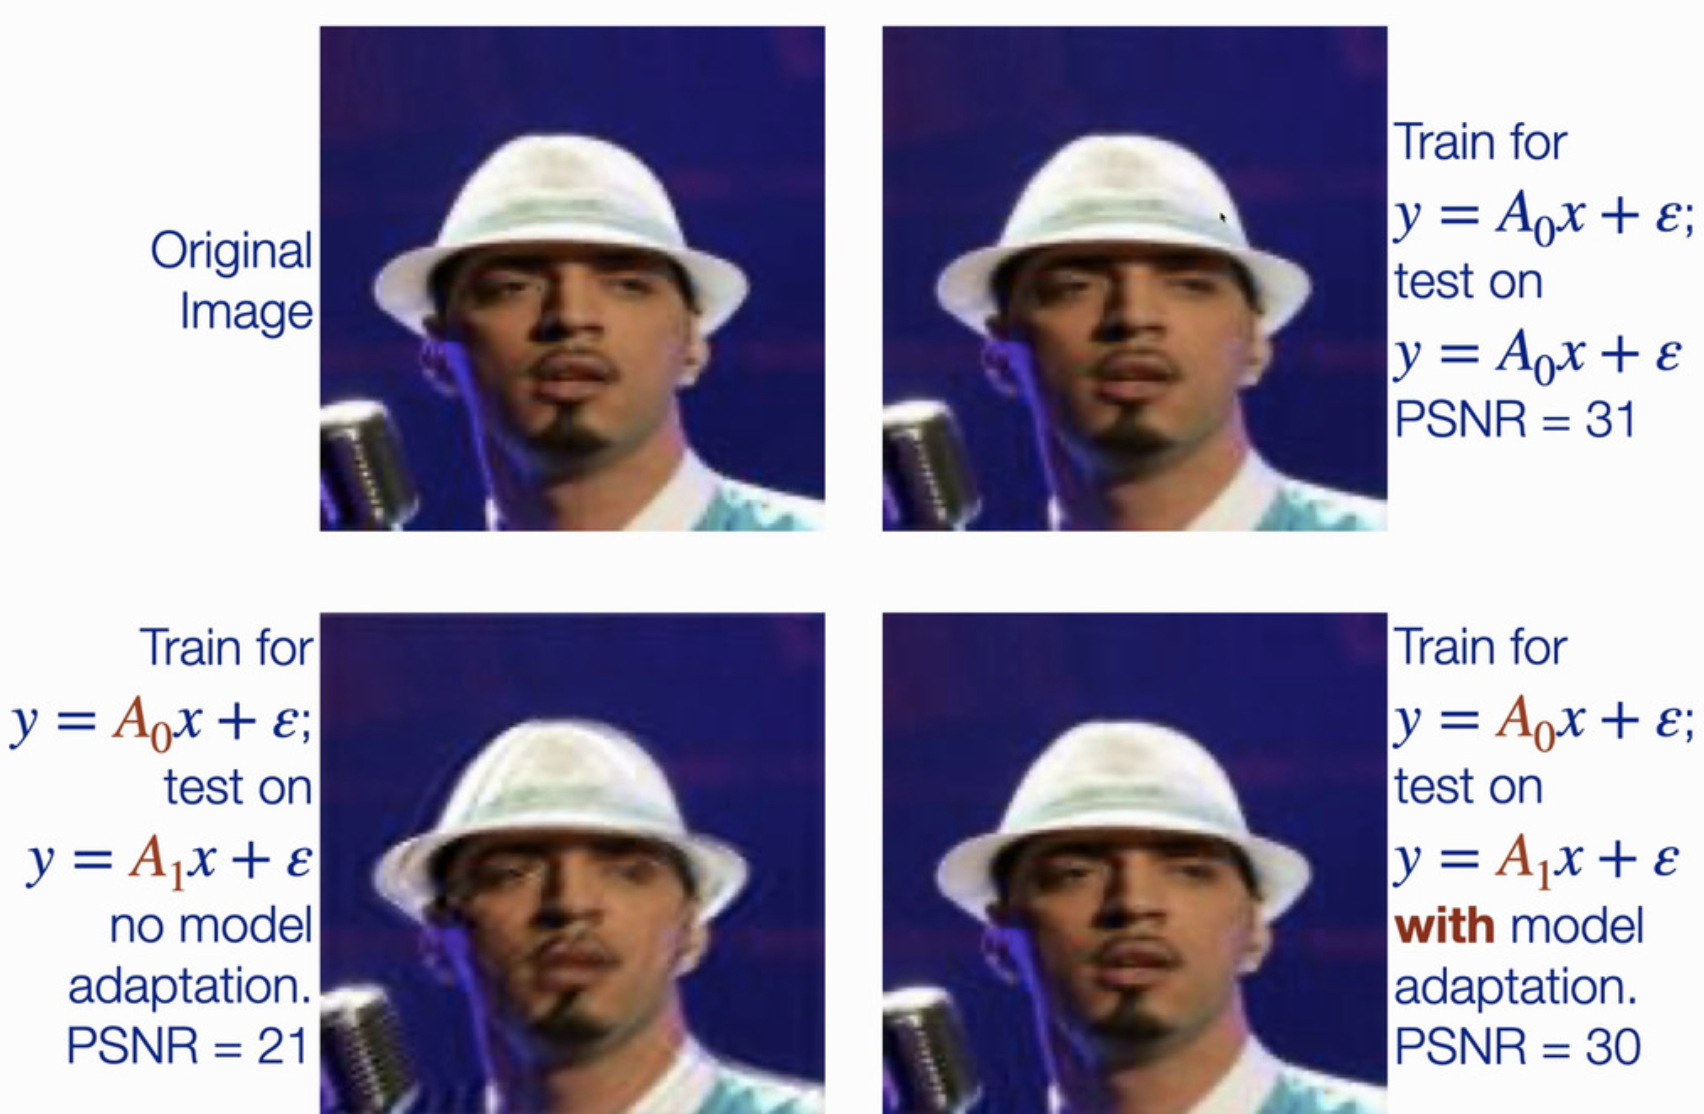
\includegraphics[scale=0.4]{neurips-2020/images/Screenshot 2020-12-13 at 21.13.52.png}
    \caption{Example of the performance of the proposed method for the general domain motion correction problem}
    \label{fig:moco_recon}
\end{figure}





\subsubsection{fastMRI}

Presented by \textit{Larry Zitnick}. \\

{\bf Motivation:} describe the fastmMRI problem, present a network by organizers of the fastMRI challenge, describe model evaluation process \\

{\bf Note:} for some reason problem of the fastMRI challenge 2019 are discussed. 
Not sure why authors did not also include discussion of this year's problem. \\

{\bf Problem:} reconstructions from the model have less noise hence look unnatural to radiologists.

{\bf Solution:} add noise to the model recons (fig. \ref{fig:smooth_fastmri}). 
This approach worked good for them (radiologists are satisfied). \\

\begin{figure}[h!]
    \centering
    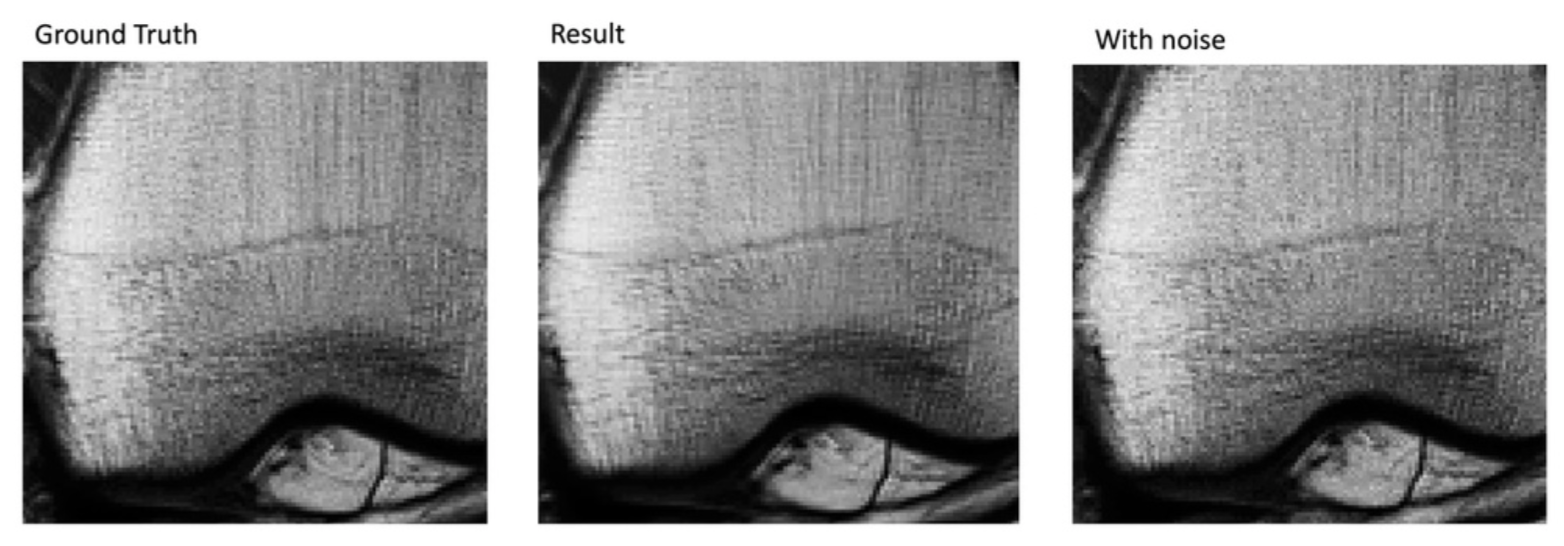
\includegraphics[scale=0.4]{neurips-2020/images/Screenshot 2020-12-13 at 22.23.29.png}
    \caption{Example of high-quality but oversmoothed result from the reconstruction model.}
    \label{fig:smooth_fastmri}
\end{figure}

{\bf Observation:} authors experienced horizontal banding artefacts (fig. \ref{fig:binding_artecats}) in their multi-coil 4x reconstructions. 
Reason - insufficient sampling pattern. 
K-space is sampled vertically (Cartesian sampling), which results in higher resolution in vertical dimension compared to the horizontal dimension and hence causing horizontal artefacts (explanation for the presenter). \\

\begin{figure}[h!]
    \centering
    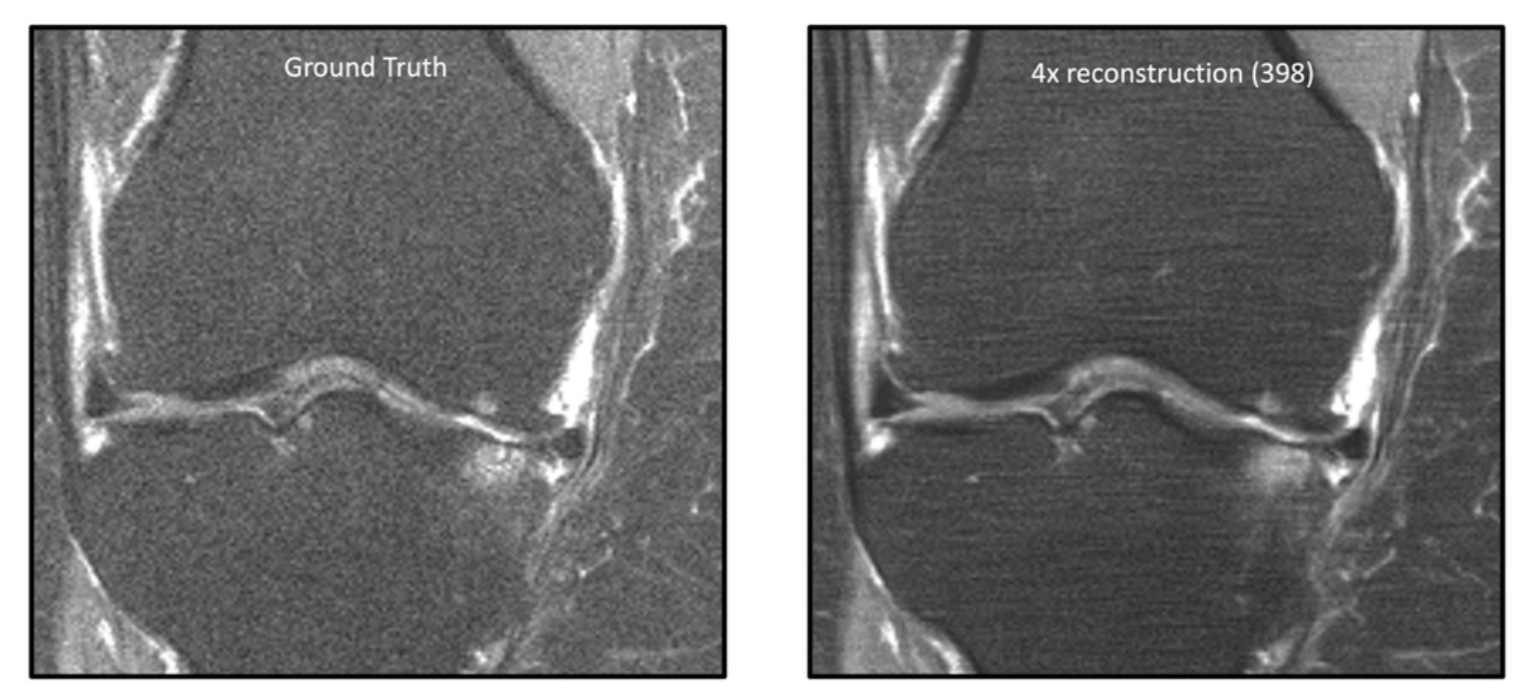
\includegraphics[scale=0.4]{neurips-2020/images/Screenshot 2020-12-13 at 22.32.40.png}
    \caption{Horizontal binding artefacts caused by insufficient sampling pattern.}
    \label{fig:binding_artecats}
\end{figure} 

{\bf Method:} most of the talk very similar to the same talk from the last year. 
The new part was the interchangeability study, which authors performed using 4x acceleration (3T) and 108 patients. 
Reconstructions were reviewed by 6 radiologists according to the following process:
\begin{itemize}
    \item Radiologist reviews a scan
    \item Waits one month
    \item Same radiologist reviews the scan
    \item Separate radiologist compares the two reports
\end{itemize} \\

{\bf Results:} in the previously described setting:
\begin{itemize}
    \item New reconstructions are diagnostically interchangeable with traditional MRIs
    \item Radiologists could not distinguish which images were produced with AI and which came from the slower traditional scans
    \item All examiners rated the AI-generated images as being higher in quality than traditional scans
\end{itemize}

Note that all these results are obtained only for a single anatomy (knee) and for a limited number of protocols (only the ones that are present in the fastMRI knee dataset).









% ------------
% -- Saturday --
% ------------
\newpage
\section{Saturday, December 12th}
\subsection{Workshop: Medical Imaging Meets NeurIPS}

\subsubsection{DeepSim: Semantic similarity metrics for learned image registration \cite{abs-2011-05735}}

Presented by \textit{Steffen Czolbe}. \\

{\bf Motivation:} having a decent solution of image registration as an ill-posed problem is heavily dependent on the presence of a meaningful distance metric $D$ (fig. \ref{fig:image_reg_problem_setting}). \\

\begin{figure}[!h]
    \centering
    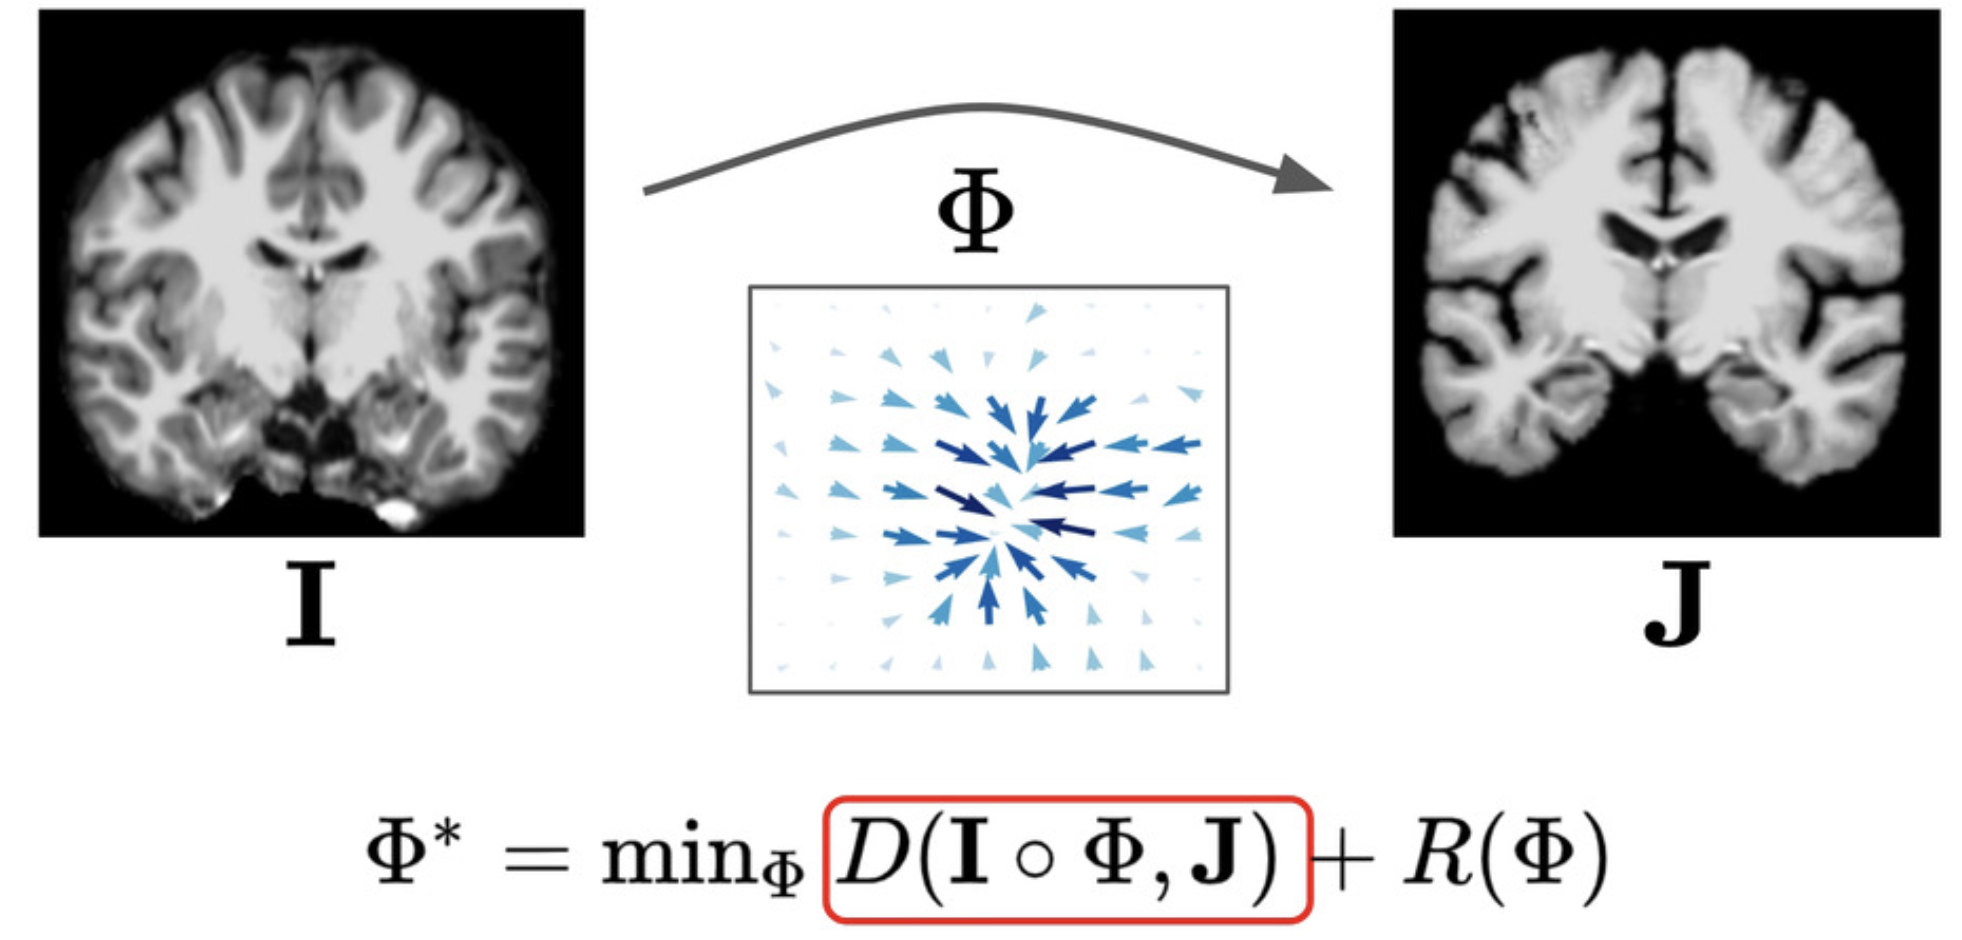
\includegraphics[scale=0.4]{neurips-2020/images/Screenshot 2020-12-15 at 16.48.59.png}
    \caption{Medical image registration problem setting. Selection of a distance metric $D$ plays a key role.}
    \label{fig:image_reg_problem_setting}
\end{figure}

{\bf Observation:} typically, the distance in image registration task is computed on patches as pixel-wise cosine distance (eq. \ref{eq:pixel_wise_cosine_distance}) between reconstruction and some generated reference.
The problem here is that pixel-wise esitmations are typically not very accurate and can be improved by replacing pixel with some more high-level features.

\begin{equation}
    NCC_{patch} (A, B) = \frac{<A - \hat{A}, B - \hat{B}>}{|| A - \hat{A} || || B - \hat{B} ||}
    \label{eq:pixel_wise_cosine_distance}
\end{equation}

{\bf Method:} pretrain some feature extractor on a proxy task withing the same imaging domain (segmentation), use its features as an enriched substitutions of raw pixel values (eq. \ref{eq:features_consine_distance}). 

\begin{equation}
    DeepSim_{patch} (A, B) = \frac{< F(A), F(B) >}{|| F(A) || || F(B) ||}
    \label{eq:features_consine_distance}
\end{equation}

{\bf Results:} as claimed:
\begin{itemize}
    \item High registration accuracy across multiple datasets
    \item The metric is general and can be applied to different modalities and algorithms 
    \itema Translations results are smoother
\end{itemize}





\subsubsection{Using StyleGANs for Visual Interpretability of Deep Learning Models on Medical Images \href{http://www.cse.cuhk.edu.hk/~qdou/public/medneurips2020/70_neurips2020_cameraready_opt.pdf}{paper}}

Presented by \textit{Kathryn Schutte}. \\

{\bf Motivation:} intractability of Machine Learning models in important, especially in medical imaging. 
The goal is to improve intractability by proposing an alternative go the currently popular GradCAM \cite{SelvarajuCDVPB17} approach. \\

{\bf Observation:} currently used methods (for example GradCAM) only highlight regions of an image that has the highest contribution to the result that a model outputs.
Instead, one could generate an image view that would lead to another output. Example is shown on the fig. \ref{fig:gradual_changes}. \\

\begin{figure}[h!]
    \centering
    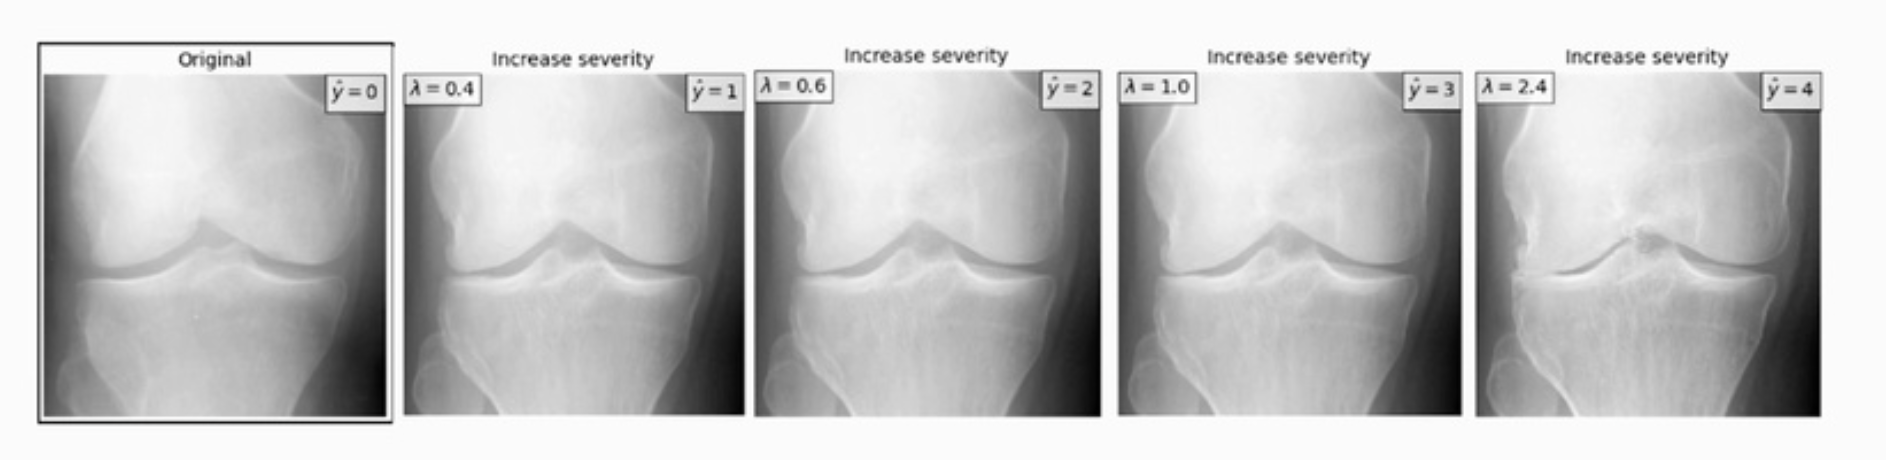
\includegraphics[scale=0.4]{neurips-2020/images/Screenshot 2020-12-15 at 20.22.51.png}
    \caption{Illustration changes of image view that could lead to a different model output. In this case classification task is considered and the initial output of the model is 0 (no pathology). However, one can have a hard time understanding why the prediction is so. For that, the proposed method generates transformations of the initial image that would lead to the alternative classification results.}
    \label{fig:gradual_changes}
\end{figure}

{\bf Method:} the following pipeline is proposed:

{\bf Step 1:} train a StyleGAN model \cite{KarrasLA19}. StyleGAN is chosen because 1) it is able to generate high-quality images and 2) has an interpretable latent space vector in the bottleneck of the generator, which can be used to generate images with desired qualities (check out StyleGAN paper for more information).

{\bf Step 2:} find the direction, which has the greatest impact on the model's output (in the particular case - on Osteoarthritis severity).

\begin{equation}
    \tilde{f} (w) = \sigma (\alpha^T \textbf{w} + \beta) \approx f(g(w))
\end{equation}

So if we approximate classifier fitting a logistic regression $f$ to this latent space we can retrieve the direction of Osteoarthritis severity using $\alpha$. 
It means, that on this stage we first build a labeled dataset of latent vectors (otherwise they are hard to interpret).

{\bf Step 3:} Encode the real images into the latent space (fig. \ref{fig:encoding_of_real_images}). \\

\begin{figure}[h!]
    \centering
    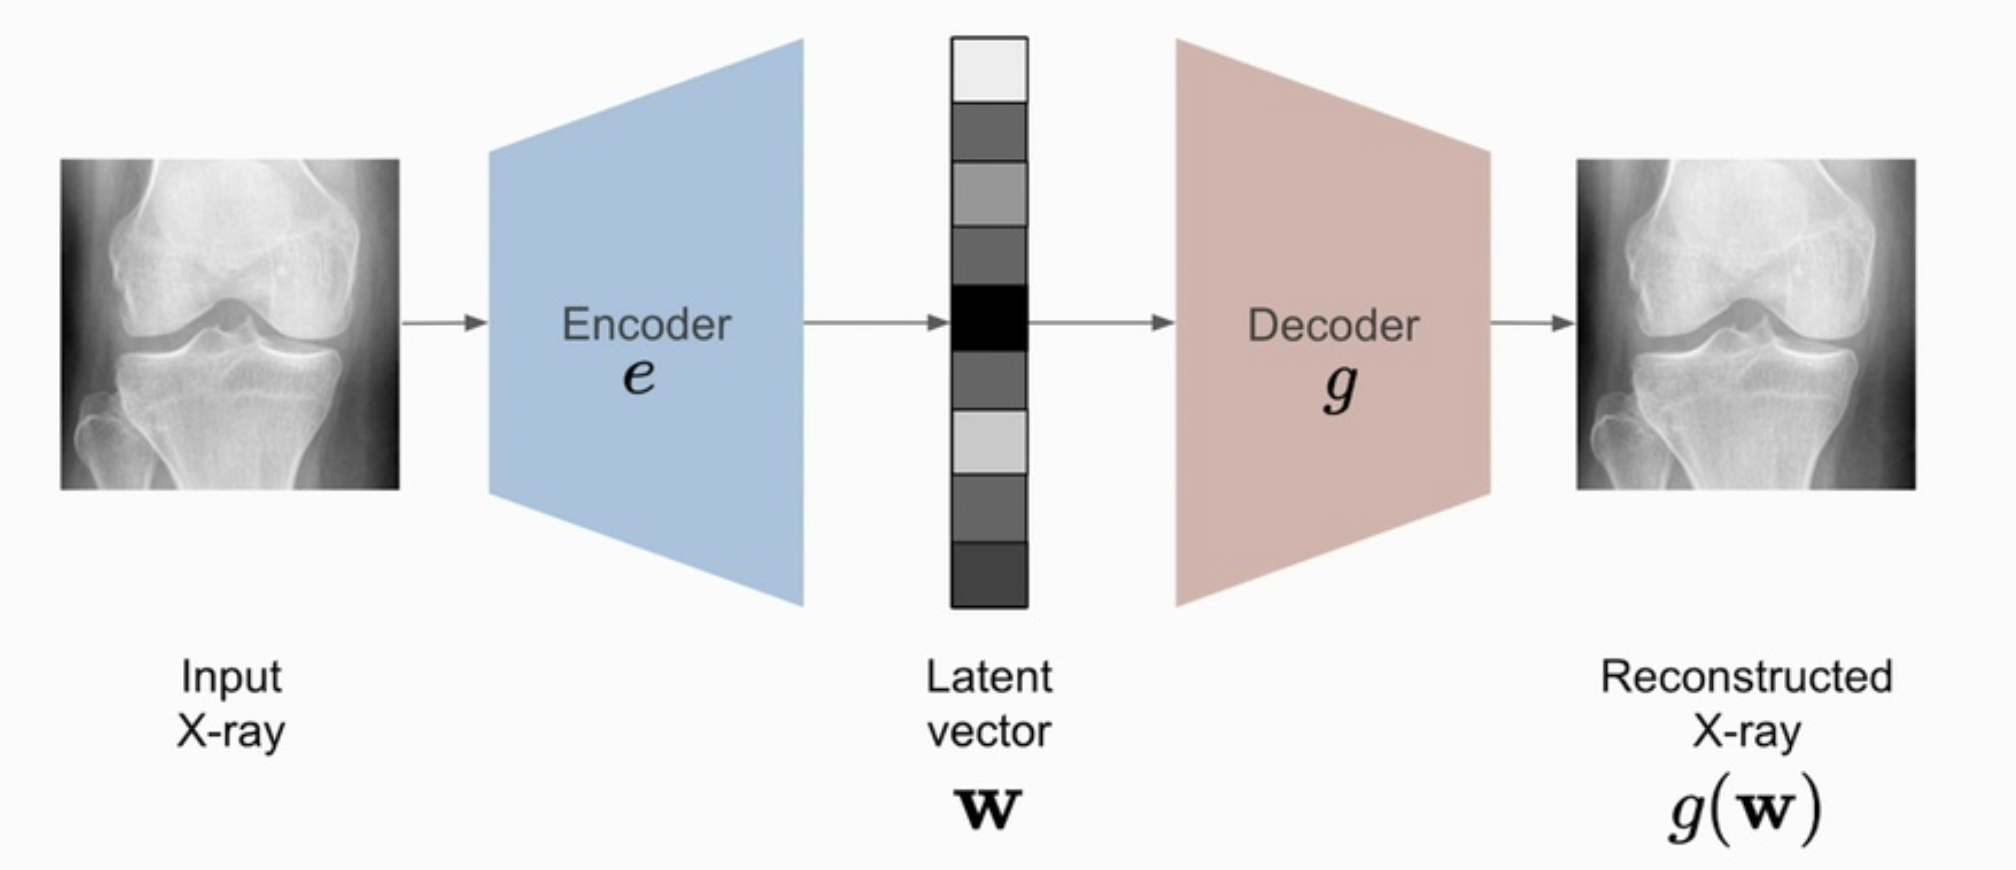
\includegraphics[scale=0.4]{neurips-2020/images/Screenshot 2020-12-15 at 20.39.44.png}
    \caption{The last step of the proposed pipeline - encoding real images into latent vectors.}
    \label{fig:encoding_of_real_images}
\end{figure}

{\bf Results:} generated images seem to be reasonable, however the solution still looks very task-specific. 
Not clear whether the proposed method will give reliable results on other domains, especially considering the fact that GAN training is in general data-hungry and available datasets may not be enough.
Also not clear how to transfer the approach for the regression task (if it is possible at all).






\subsubsection{FastMRI keynote: Fast(er) MRI: a radiologist's perspective}

Presented by \textit{Yvonne Lui}. \\

{\bf Motivation:} discuss results of this year's challenge, compare them with the ones from the previous year. \\

{\bf Observation:} organizers claim that overall SSIM has a decent correlation with radiologist's rankings of challenge results. 
More concretely, when SSIM values are very different, their relative order well correlates with the order provided my manual evaluations with radiologists.
However, when differences in values are small (3rd-4th digit), like we can commonly observe in top-3 of the leaderboard, relative order may be different. 
In particular, top-2 and top-3 results (according to their SSIM scores, difference in the 3rd digit) were flipped after evaluation from radiologists. \\

{\bf Observation:} top-3 values of SSIM scores from 2020 challenge are much higher than corresponding values from the previous year.
2019 winner would not get into top-3 in 2020 with the same SSIM score. 
However, it is not clear whether such a direct comparison is fair due to the fact that 2019 and 2020 challenges utilized very different data (different anatomies, protocols). \\

{\bf Observation:} last year's manual evaluation procedure was not aimed at finding the most accurate (from the anatomical perspective) reconstructions.
Instead, radiologists only judged on the perceptual feeling of quality, which led to the problem illustrated on fig. \ref{fig:2019_problems}. 
Here, none of the reconstructions was good enough to capture the important anatomical structure while radiologists ranked all these reconstructions to be high-quality. \\

\begin{figure}[h!]
    \centering
    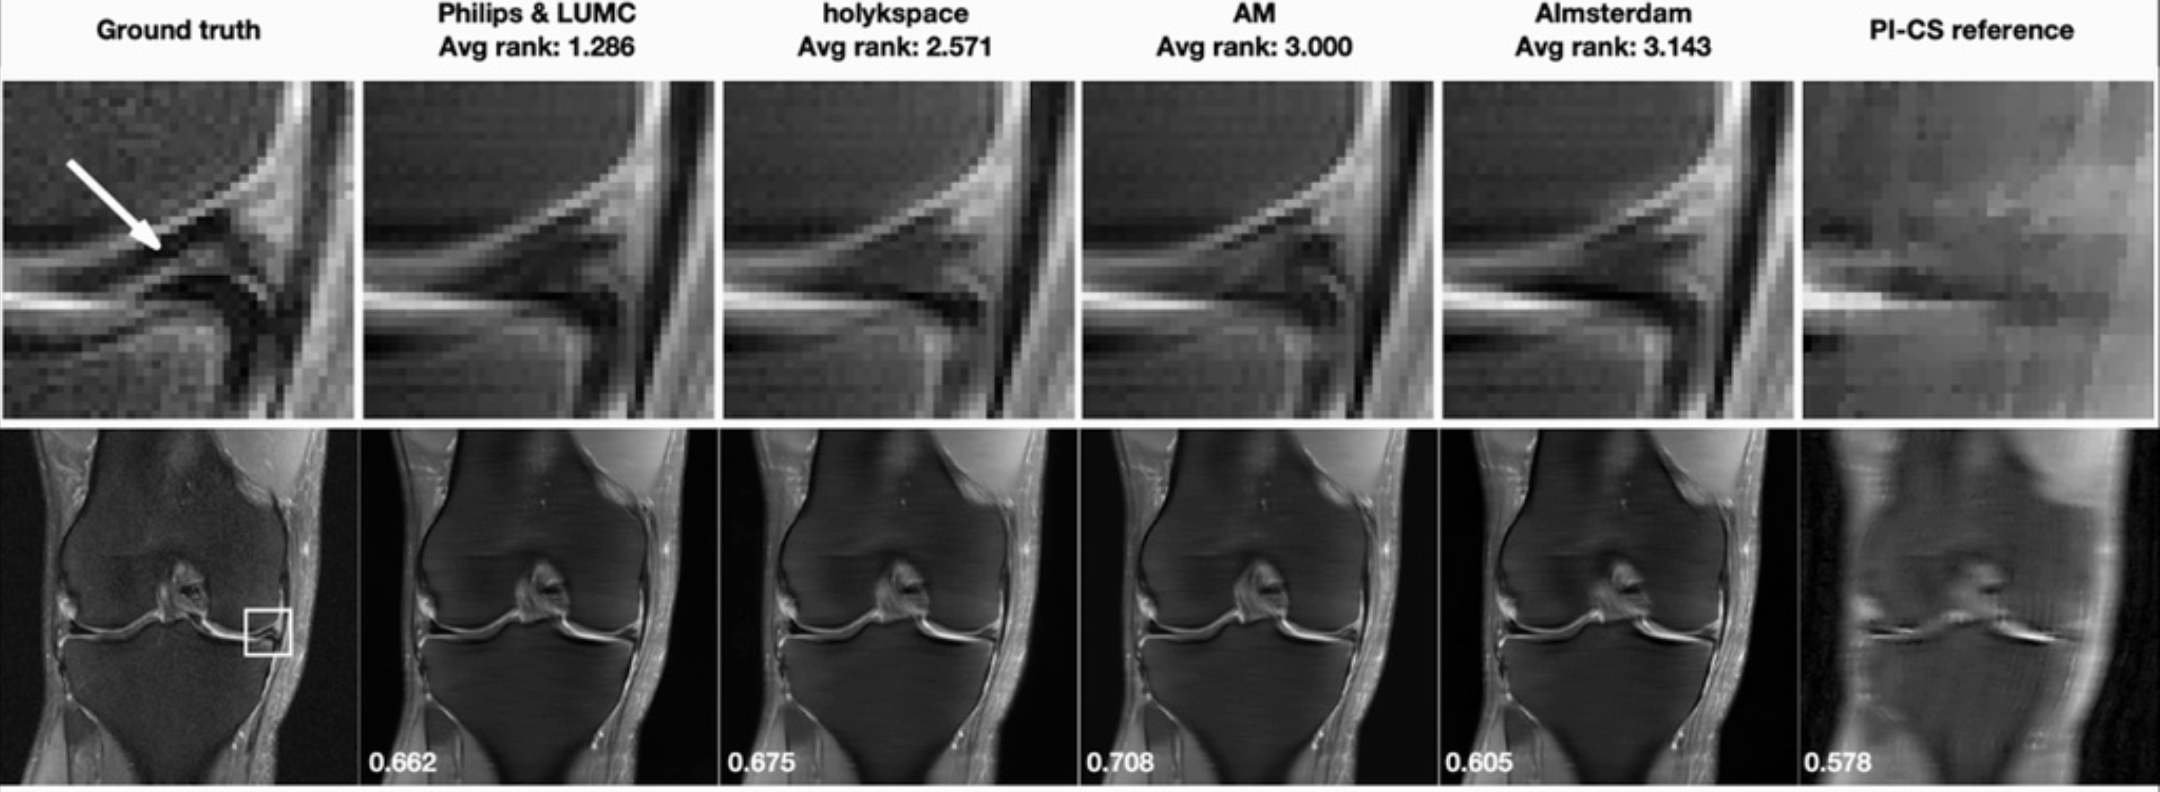
\includegraphics[scale=0.4]{neurips-2020/images/Screenshot 2020-12-15 at 11.17.48.png}
    \caption{Example from the 2019 challenge, when all reconstructions failed to preserve an important anatomical structures but still were hightly ranked by experts.}
    \label{fig:2019_problems}
\end{figure}

To avoid the same problem this year, organizers revised the evaluation process and carefully selected several pathologies. \\

{\bf New evaluation process:} radiologist were asked to rank reconstructions by assigning them scores from 1 to 4, where lower is better in for different criteria: presence of artefacts, sharpness and contrast-to-noise ratio (CNR). \\

{\bf Multi-coil 4x and 8x tracks:} this is very similar challenge to the 2019 version except from data and the evaluation process. 
The presentation of results of showed that 8x acceleration is still to high for a potential clinical application with diagnostic purposes. \\

{\bf Transfer track:} this track was aimed to estimate how good model trained on data from one vendor can be used on data from another vendors.
In particular Siemens data was used for training and transferring was tested on GE and Philips data.
Overall, Philips appeared to be closer to Siemens data resulting in (in general) better reconstructions. 
However, results greatly vary depending on contrast and particular anatomical structures.

{\bf Note:} one of competitors this year also provided estimates of coil sensitivity maps (CSMs) as a part of their submission.
This could help them to increase the overall quality (not clear whether it helped a lot though).

{\bf Note:} presented mentioned the work from MRM (early 2020) on Gibbs deringing \cite{Muckley_2020} where authors were able to create a system for Gibbs ringing removing. The artefacts were result of a partial Fourier transform.
They did it by training a neural network on ImageNet dataset for the deringing task. 
Then this model was applied to MRI data and showed a decent performance. \\





% ----------------------
% -- Acknowledgements --
% ----------------------
\section{Acknowledgements}
I’d like to acknowledge the assistance of Mikhail Bortnikov who was helping me to not miss the most interesting parts of the conference, live poster presentations and tutorials. 


% --- Bibliography ---
\newpage
\bibliographystyle{plainnat}
\bibliography{bibliography}

\end{document}
